\clearpage
\bookpart{分块优化}{Block Optimization}
\label{part:block-optimization}

\BookPartGuide{%
许多问题的变量维数很高，但固定其余变量后，只对一部分变量求解却很便宜。按块更新正是利用这一点：每次只动一块变量，用较小的代价换取完整目标的进展。

第~\ref{chap:block-optimization}章先建立块坐标下降的共同框架，比较循环、随机和贪心的选块方式，再按块内的计算手段组织算法：精确求解条件子问题、最小化局部模型、使用块邻近更新以及交替求解矩阵因子。逐块最优并不等于整体最优，章中用反例说明这一差距，并给出保证完整目标进展所需要的条件。}

\chapter{分块优化}
\label{chap:block-optimization}

设想一个有一百万列的最小二乘问题。每算一次完整梯度，都要把矩阵的全部元素读一遍。如果其他变量都不动，只调整一个系数，那么最优的调整量只用这一列就能算出来。再设想把一张评分表分解成两个因子的乘积：同时求两个因子是非凸问题，但固定其中一个，另一个就是普通的最小二乘。两个问题有同一个特点：变量合在一起很难处理，拆开之后每一部分都便宜。

本章研究这种“每次只处理一部分变量”的做法。核心问题有两个：只动一部分变量，能不能保证完整目标取得进展？这样省下来的计算，会不会被更多的迭代次数抵消？

第~\ref{sec:block-problem}节先说明怎样划分变量，以及哪些耦合会让逐块更新寸步难行。第~\ref{sec:block-bcd}节以精确求解一块为基准，建立选块的三种规则。精确求解常常太贵，第~\ref{sec:block-local}节改用局部模型，并给出加速和曲率的版本。第~\ref{sec:block-alternating}节研究变量自然分成少数几组的情形，以矩阵分解为主例，同时看到逐块最优的局限。

这些方法看上去各不相同，第~\ref{sec:block-bsum}节用“块上界”解释它们中的一大部分为什么能下降，第~\ref{sec:block-bpg}节把这一想法用到带非光滑项的目标上。第~\ref{sec:block-implementation}节把算法放回实际计算：并行时步长怎样改，子问题要解到多准，各种保证分别回答什么问题，总工作量是否真的减少。

\section{分块问题}
\label{sec:block-problem}

本节回答一个问题：把变量分成若干块、每次只动一块时，块应当怎样划分，块与块之间的哪些关系会妨碍这种做法。

\subsection{块的划分}
\label{sec:block-partition}

\paragraph{两个具体的问题}
先看最小二乘。设$\bm{A}\in\mathbb{R}^{N\times n}$，第$j$列记为$\bm{a}_j$，目标是
\[
 f(\bm{x})=\frac12\lVert\bm{A}\bm{x}-\bm{b}\rVert_2^2 .
\]
若其他系数不动，只改$x_j$，残差$\bm{r}=\bm{A}\bm{x}-\bm{b}$只沿$\bm{a}_j$变化。这时一列数据就够用，变量的一个分量自然成为一块。

再看矩阵分解。给定$\bm{Y}\in\mathbb{R}^{p\times q}$，寻找$\bm{U}\in\mathbb{R}^{p\times r}$、$\bm{V}\in\mathbb{R}^{q\times r}$，使$\bm{U}\bm{V}^\top$接近$\bm{Y}$，目标是
\[
 \lVert\bm{Y}-\bm{U}\bm{V}^\top\rVert_F^2 .
\]
这里最自然的一块不是单个元素，而是整个因子。固定$\bm{V}$后，目标关于$\bm{U}$是凸二次的，可以一次解出。

\paragraph{块与条件子问题}
两个例子的共同结构是：把坐标分成互不重叠的几组，每次只让一组变化。为了精确地谈论这件事，需要一套记号。

\begin{definition}[变量分块与条件子问题]
\label{def:block-partition}
把下标集$\{1,\ldots,n\}$划分为$B$个互不相交的非空子集$J_1,\ldots,J_B$，每个子集称为一个\term{变量块}（variable block）。对块$J$，记$\bm{x}_J\in\mathbb{R}^{\lvert J\rvert}$为$\bm{x}$在$J$上的分量，$\bm{U}_J\in\mathbb{R}^{n\times\lvert J\rvert}$为单位矩阵中由$J$对应的列组成的子矩阵，并记偏梯度
\begin{equation}
 \nabla_Jf(\bm{x})=\bm{U}_J^\top\nabla f(\bm{x}).
 \label{eq:block-partial-gradient}
\end{equation}
固定$\bm{x}$在其他块上的取值，把块$J$的取值换成$\bm{z}$，得到的函数
\begin{equation}
 \varphi_J(\bm{z};\bm{x})=f\bigl(\bm{x}+\bm{U}_J(\bm{z}-\bm{x}_J)\bigr)
 \label{eq:block-conditional}
\end{equation}
称为块$J$的\term{条件函数}（conditional function），在块$J$的允许集合上最小化它的问题称为\term{条件子问题}（conditional subproblem）。
\end{definition}

$\bm{U}_J\bm{h}$的作用是把长度为$\lvert J\rvert$的向量$\bm{h}$放回块$J$的位置，其余分量补零。单个坐标是块大小为$1$的特殊情形，下文的结论同时覆盖单坐标和多坐标的块。图~\ref{fig:block-columns-rows}(a)是这种划分的样子：绿色的一段正在变化，其余两段被固定。

\begin{BookInlineFigure}
  \centering
  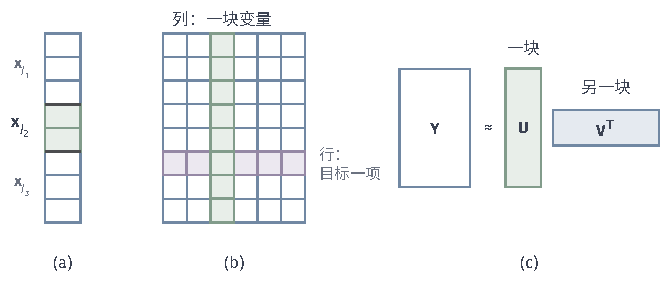
\includegraphics[width=112mm]{figures/05-optimization/04-block-optimization/tikz/block-columns-rows/figure.pdf}
  \caption{变量分块的三种形式。(a)向量$\bm{x}$分成三块，绿色的块$J_2$正在更新，其余块固定。(b)最小二乘的数据矩阵：选一列（绿）是选一块变量；选一行（紫）是选目标的一项，后者不属于本章的做法。(c)矩阵分解中，整个因子$\bm{U}$是一块。}
  \label{fig:block-columns-rows}
\end{BookInlineFigure}

图~\ref{fig:block-columns-rows}(b)还指出了一个容易混淆的区别。选列是在变量上做选择，读到的偏导数是准确的；选行是在目标的求和项上做选择，读到的方向只是全梯度的一个估计。两种选择回答不同的问题，也可以组合使用。选行带来的方向误差留到第~\ref{chap:stochastic-gradient-methods}章研究，本章的偏梯度都是精确的。

\paragraph{贯穿本章的例子}
全章反复使用同一个带交叉项的二元二次目标，起点固定为$(3,4)$：
\begin{equation}
 f(\bm{x})=x_1^2+x_1x_2+x_2^2,\qquad \bm{x}^{(0)}=(3,4).
 \label{eq:block-example}
\end{equation}
它的梯度和Hessian分别是
\[
 \nabla f(\bm{x})=\begin{bmatrix}2x_1+x_2\\x_1+2x_2\end{bmatrix},\qquad
 \bm{Q}=\begin{bmatrix}2&1\\1&2\end{bmatrix}.
\]
$\bm{Q}$的特征值是$1$和$3$，所以强凸常数$\mu=1$，光滑常数$L=3$，唯一的最优解是原点，$f^\star=0$。起点的目标值是
\[
 f(\bm{x}^{(0)})=9+12+16=37 .
\]

这个目标也是一个最小二乘问题。取
\[
 \bm{A}=\begin{bmatrix}1&1\\1&0\\0&1\end{bmatrix},\qquad \bm{b}=\bm{0},
\]
则$\bm{A}^\top\bm{A}=\bm{Q}$，并且$\tfrac12\lVert\bm{A}\bm{x}\rVert_2^2$展开后正是式~\eqref{eq:block-example}。对一般的$\bm{b}=\bm{A}\bm{x}^\star$，把变量平移成$\bm{x}-\bm{x}^\star$就回到$\bm{b}=\bm{0}$，这里取$\bm{0}$只是为了算起来干净。

\paragraph{一个坐标还是两个一起}
现在比较两种走法。按坐标更新时，把$x_2=4$固定，条件函数$z^2+4z+16$在$z=-2$取最小，走到$(-2,4)$；再固定$x_1=-2$，走到$(-2,1)$。

联合求解则把两个变量当成一块，解方程$\bm{Q}\bm{x}=\bm{0}$，一步到达原点。下表记录了目标值，图~\ref{fig:block-joint-vs-coordinate}是对应的路径。

\begin{BookInlineTable}
\centering
\begin{tabular}{lcc}
\toprule
做法 & 计算量 & 走完后的目标值\\
\midrule
更新$x_1$ & 一次除法 & $12$\\
再更新$x_2$ & 一次除法 & $3$\\
联合求解 & 解一个$2\times2$方程组 & $0$\\
\bottomrule
\end{tabular}
\end{BookInlineTable}

\begin{BookInlineFigure}
  \centering
  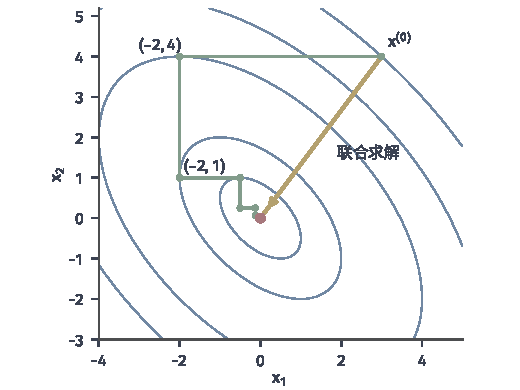
\includegraphics[width=88mm]{figures/05-optimization/04-block-optimization/matplotlib/block-joint-vs-coordinate/figure.pdf}
  \caption{式~\eqref{eq:block-example}上坐标更新与联合求解的比较。蓝色是等高线，绿色折线是依次精确更新$x_1$、$x_2$的前三轮，只能沿坐标轴方向走；黄色箭头是把两个变量当作一块、一步解出的路径；红点是最优解。}
  \label{fig:block-joint-vs-coordinate}
\end{BookInlineFigure}

块越大，每步的进展越大，但一步也越贵。这个交换关系在高维时才真正显出来。图~\ref{fig:block-size-cost}取$n=64$的链式二次目标，Hessian为三对角矩阵，主对角线上是$2.02$，次对角线上是$-1$，把相邻的$p$个变量分成一块，依次精确求解。

\begin{BookInlineFigure}
  \centering
  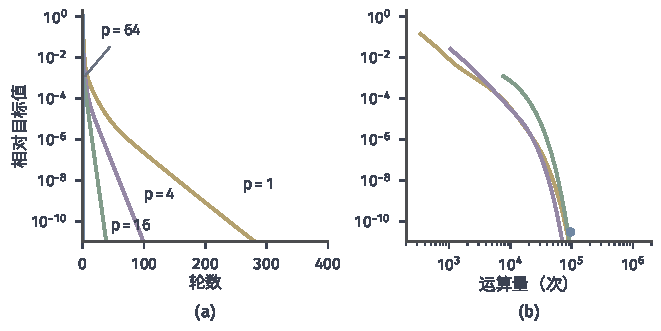
\includegraphics[width=112mm]{figures/05-optimization/04-block-optimization/matplotlib/block-size-cost/figure.pdf}
  \caption{块大小与计算量的交换。目标是$n=64$的链式二次函数，$p$个相邻变量为一块，循环精确更新。(a)相对目标值随轮数的变化，块越大轮数越少，$p=64$一轮即解出。(b)同一组数据按运算量画出，颜色与(a)相同，运算量按稠密块计：每块一次Cholesky分解计$p^3/3$，每次回代计$2p^2$，读取耦合项计$3p$，蓝点是$p=64$一次解出所用的运算量。}
  \label{fig:block-size-cost}
\end{BookInlineFigure}

以相对目标值降到$10^{-10}$为准，从(a)看，把块从$1$增大到$16$，所需轮数从$239$减到$34$，好像块越大越好。(b)把横轴换成运算量后，优势大半消失：四种块大小的总运算量都在$6\times10^4$到$10^5$之间，$p=4$反而最少。块大了一轮贵得多，轮数减少的好处被抵消了。选择块大小时，不能只看轮数。

\paragraph{决定块大小的三件事}
由此可以归纳出三个需要同时考虑的因素。第一是变量耦合：彼此强耦合的变量放进同一块，块内的联合求解才能消除这种耦合。第二是子问题的求解：块内要有闭式解、可复用的分解或便宜的迭代，否则分块省不下计算。

第三是数据读取：一块对应的数据最好能连续读取，并能借助残差之类的中间量增量维护，否则每次更新一块也要把数据读遍。

无论块怎样划分，评价进展时都看完整目标$f$，而不是当前块上条件函数的值。条件函数的最小值只说明这一块调到了最好，并不说明问题解决了。第~\ref{sec:block-exact}小节会用数字说明这个区别。

\subsection{块间耦合}
\label{sec:block-coupling}

上一小节的耦合只影响速度。有些耦合更严重，它让逐块更新根本走不动。本小节看两种情形，它们决定了后面每个算法都要检查的两个条件：可行性和可分性。

\paragraph{乘积可行域}
若可行集是各块集合的乘积
\begin{equation}
 \bm{C}=\bm{C}_{J_1}\times\cdots\times\bm{C}_{J_B},
 \label{eq:block-product-set}
\end{equation}
每一块只需留在自己的集合内，整个点就是可行的。各块的约束互不牵连，逐块更新可以自由进行。箱式约束$l_j\leq x_j\leq u_j$是最常见的例子，图~\ref{fig:block-feasible-coupling}(a)中沿任一坐标轴移动，只要不越过自己的边界，点就留在矩形内。

\paragraph{耦合约束}
情况在约束把几块绑在一起时完全不同。设$\bm{x}\in\mathbb{R}^n$满足$\sum_{j=1}^nx_j=1$，可行点$\bm{x}$的$x_j$改成$x_j+\delta$，分量之和就变成$1+\delta$。所以只要$\delta\neq0$就不可行，单坐标更新只能停在原地。

要在这个集合内移动，至少同时改两个坐标，让它们的变化互相抵消：
\[
 x_i\leftarrow x_i+\delta,\qquad x_j\leftarrow x_j-\delta .
\]
图~\ref{fig:block-feasible-coupling}(b)画出$n=3$的情形。红色的单坐标方向离开了三角形所在的平面，绿色的两坐标方向留在平面内。

\begin{BookInlineFigure}
  \centering
  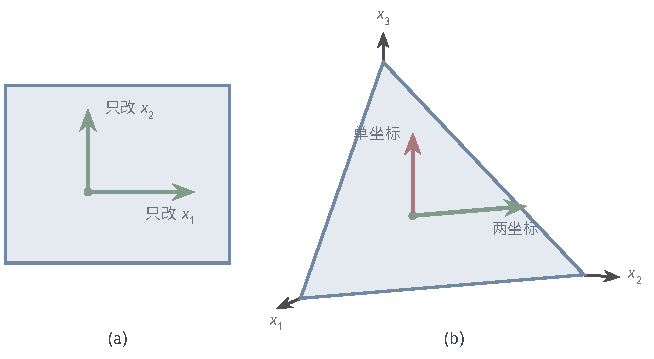
\includegraphics[width=108mm]{figures/05-optimization/04-block-optimization/tikz/block-feasible-coupling/figure.pdf}
  \caption{可行域与块的移动。(a)乘积可行域：矩形内的点沿任一坐标轴移动都可以留在可行域内。(b)$\sum_jx_j=1$的可行点（只画$x_j\geq0$的部分）：红色的单坐标移动离开平面，变得不可行；绿色的两坐标移动保持分量之和不变。}
  \label{fig:block-feasible-coupling}
\end{BookInlineFigure}

一般的耦合约束需要借助乘子把它们拆开，这部分内容放在第~\ref{chap:penalty-multiplier-methods}章。本章只讨论乘积可行域。

\paragraph{不可分的非光滑项}
另一种障碍来自目标本身。考虑凸函数
\begin{equation}
 F(u,v)=2\lvert u-v\rvert+\lvert u+v-2\rvert ,
 \label{eq:block-nonsmooth-example}
\end{equation}
它的最小值在$(1,1)$处取到，$F(1,1)=0$。把点放在原点，$F(0,0)=2$，看两个坐标方向能否改进。

固定$v=0$，条件函数是$F(u,0)=2\lvert u\rvert+\lvert u-2\rvert$，分段写出来就是
\[
 F(u,0)=\begin{cases}
 2-3u, & u<0,\\
 2+u, & 0\leq u\leq2,\\
 3u-2, & u>2.
 \end{cases}
\]
左边斜率为负，右边斜率为正，所以$u=0$是唯一的最小点。由$F$关于$u,v$的对称性，固定$u=0$时$v=0$也是唯一的最小点。

因此从原点出发，两个坐标都不肯动，算法永远停在目标值$2$处。可是沿对角线走却能下降：
\[
 F(s,s)=2\lvert s-1\rvert ,
\]
$s$从$0$增大到$1$时目标值从$2$降到$0$。图~\ref{fig:block-nonsmooth-stall}画出了这一情形。

\begin{BookInlineFigure}
  \centering
  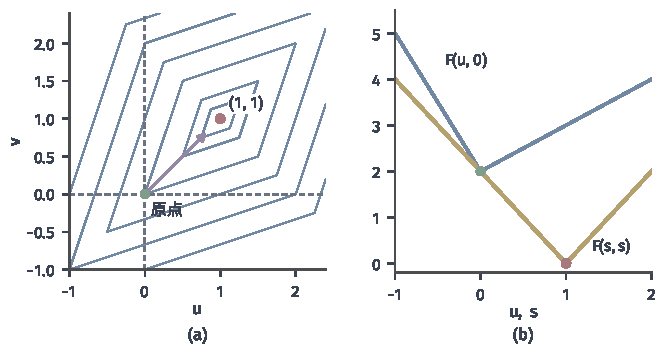
\includegraphics[width=112mm]{figures/05-optimization/04-block-optimization/matplotlib/block-nonsmooth-stall/figure.pdf}
  \caption{不可分非光滑项造成的坐标停滞。$F(u,v)=2\lvert u-v\rvert+\lvert u+v-2\rvert$。(a)蓝色是等高线，它们在折线上有尖角。绿点是原点，两条灰色虚线是过原点的坐标方向，紫色箭头指向最优解（红点）。(b)蓝线是坐标方向上的$F(u,0)$，在原点取最小；黄线是对角线方向上的$F(s,s)$，从原点继续下降。}
  \label{fig:block-nonsmooth-stall}
\end{BookInlineFigure}

原因在于原点恰好落在折线$u=v$上。原点附近$u+v-2<0$，于是
\[
 F(u,v)=2\lvert u-v\rvert+2-u-v .
\]
方向$(d_1,d_2)$要下降，必须满足$2\lvert d_1-d_2\rvert<d_1+d_2$，这些方向夹在$(3,1)$和$(1,3)$之间，是以对角线为中心的一个窄角，两个坐标方向都在窄角之外。

可以想象站在一条斜向的沟底，沿沟走是下坡，朝东西或南北走都会撞上沟壁。这个类比只对应“沿坐标方向不能下降”这一点：沟底是目标的尖角，光滑的目标没有这样的沟壁。如果$F$可微，两个偏导数都为零意味着梯度为零，这种事就不会发生。

这两种情形提醒我们，后面每个算法都要回答两个问题：只改一块时点还可行吗？非光滑项能按块拆开吗？第~\ref{sec:block-limits}小节还会回到这个反例，把“每块都不能改进”与“整体最优”的差别说清楚。

\section{块坐标下降（BCD）}
\label{sec:block-bcd}

上一节把变量分成了块。接下来要弄清：每次选一块、固定其余变量并改善完整目标，这个过程应当怎样组织？

\term{块坐标下降}（block coordinate descent，BCD）把一次迭代拆成两个环节：选块决定这一步动哪一块，块内更新决定这一块怎样动。两个环节可以自由搭配。本节先固定块内更新为“精确求解条件子问题”，集中比较循环、随机、贪心三种选块方式；第~\ref{sec:block-local}节以后再替换块内更新。

这些选块规则也能用于后面的梯度、邻近或模型更新，但搭配之后的下降和收敛保证要重新核对，不能直接搬用。

\subsection{精确块更新}
\label{sec:block-exact}

\paragraph{更新规则}
设可行集是乘积形式~\eqref{eq:block-product-set}，当前点为$\bm{x}^{(t)}$，选中块$J$。精确块更新在块$J$的允许集合上最小化条件函数，其他块不动：
\begin{equation}
 \bm{x}_J^{(t+1)}\in\argmin_{\bm{z}\in\bm{C}_J}\varphi_J(\bm{z};\bm{x}^{(t)}),\qquad
 \bm{x}_{i}^{(t+1)}=\bm{x}_{i}^{(t)}\ \ (i\notin J).
 \label{eq:block-exact}
\end{equation}
这里的“$\in$”提醒我们最小点可能不止一个。

\paragraph{完整目标不增}
这个规则带来的进展来自一个简单的比较：当前的$\bm{x}_J^{(t)}$本身就是子问题的一个候选，最优解不会比它差。其他块又没有改变，所以条件函数的值就是完整目标的值。

\begin{lemma}[精确块更新的单调性]
\label{lem:block-exact-descent}
设可行集有乘积结构~\eqref{eq:block-product-set}，$\bm{x}^{(t)}\in\bm{C}$，且条件子问题的最小点存在。按式~\eqref{eq:block-exact}更新后$\bm{x}^{(t+1)}\in\bm{C}$，并且
\begin{equation}
 f(\bm{x}^{(t+1)})\leq f(\bm{x}^{(t)}).
 \label{eq:block-exact-monotone}
\end{equation}
\end{lemma}

\begin{proof}
其他块未变，块$J$落在$\bm{C}_J$内，乘积结构保证新点可行。$\bm{x}_J^{(t)}\in\bm{C}_J$是条件子问题的可行点，最小点的函数值不超过它的函数值，于是
\[
 \varphi_J(\bm{x}_J^{(t+1)};\bm{x}^{(t)})\leq\varphi_J(\bm{x}_J^{(t)};\bm{x}^{(t)}).
\]
由定义~\eqref{eq:block-conditional}，左边等于$f(\bm{x}^{(t+1)})$，右边等于$f(\bm{x}^{(t)})$。
\end{proof}

\paragraph{两件要先核对的事}
引理假定最小点存在，这一条并非总成立。取$f(x_1,x_2)=e^{x_1}+x_2^2$，固定$x_2$后，条件函数沿$x_1\to-\infty$递减而取不到最小值，更新规则根本没有定义。使用精确块更新前，要用条件函数的紧下水平集之类的条件确认最小点存在。

最小点也可能不唯一。取$\tfrac12(uv-1)^2$，固定$v=0$时，条件函数恒等于$\tfrac12$，每个$u$都是最小点。这时算法必须事先规定怎样选，常见的规则有“当前值已是最小点就不动”或“取离当前点最近的最小点”。没有这样的规则，迭代序列就没有确定的含义，第~\ref{sec:block-convergence}小节会看到，解的选择还影响收敛结论。

\paragraph{二次目标的块解}
对二次目标，条件子问题有显式解。设
\[
 f(\bm{x})=\frac12\bm{x}^\top\bm{Q}\bm{x}-\bm{b}^\top\bm{x},
\]
其中$\bm{Q}$对称，块$J$的主子矩阵$\bm{Q}_{J,J}$正定，$\bar{J}$是$J$的补集。令偏梯度为零，
\[
 \bm{Q}_{J,J}\bm{x}_J+\bm{Q}_{J,\bar{J}}\bm{x}_{\bar{J}}-\bm{b}_J=\bm{0},
\]
解出
\begin{equation}
 \bm{x}_J^{+}=\bm{Q}_{J,J}^{-1}\bigl(\bm{b}_J-\bm{Q}_{J,\bar{J}}\bm{x}_{\bar{J}}\bigr).
 \label{eq:block-quadratic-solve}
\end{equation}

在式~\eqref{eq:block-example}中更新$x_1$。固定$x_2=4$，条件函数是
\[
 \varphi(z)=z^2+4z+16,
\]
令导数$2z+4=0$，得到
\[
 z=-2,\qquad \varphi(-2)=12 .
\]

条件子问题已经精确解出，$x_1$在固定$x_2=4$时不可能更好了。但点$(-2,4)$不是原问题的解，它的目标值是$12$，而$f^\star=0$；它的梯度也不为零：
\[
 \nabla f(-2,4)=(0,\,6).
\]
第一个分量为零，说明$x_1$这一块确实调好了；第二个分量不为零，说明$x_2$还没有。图~\ref{fig:block-exact-slice}把这两件事画在一起。

\begin{BookInlineFigure}
  \centering
  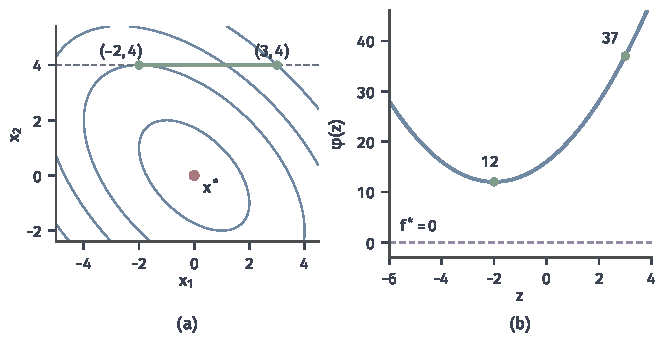
\includegraphics[width=112mm]{figures/05-optimization/04-block-optimization/matplotlib/block-exact-slice/figure.pdf}
  \caption{精确解条件子问题与解出整个问题的差别。(a)固定$x_2=4$（灰色虚线），在这条直线上从$(3,4)$移到条件最小点$(-2,4)$，该点处等高线与虚线相切，但离红色的最优解还远。(b)沿虚线的条件函数$\varphi(z)=z^2+4z+16$，绿点的值从$37$降到$12$；紫色虚线是完整问题的最优值$0$。}
  \label{fig:block-exact-slice}
\end{BookInlineFigure}

\subsection{循环块坐标下降（Cyclic BCD）}
\label{sec:block-cyclic}

\paragraph{主要思想}
最朴素的选块方式是按固定顺序轮流，这就是\term{循环块坐标下降}（cyclic block coordinate descent）。依次把$J_1,\ldots,J_B$各更新一次称为一\term{轮}（epoch）。后面的块读取的是本轮已经更新的新值，这一点很关键：刚得到的信息立刻被用上。

对二次目标，单坐标的循环更新就是线性方程组的Gauss--Seidel迭代，其收敛条件和误差传播的矩阵形式，可参考\BookChapterRef{chap:stationary-iterations}{卷二第14章“定常迭代法”}。这里我们关心的是耦合怎样决定速度。

把式~\eqref{eq:block-example}中的交叉项系数换成参数$c$，$\lvert c\rvert<2$，考虑
\begin{equation}
 f_c(\bm{x})=x_1^2+cx_1x_2+x_2^2 .
 \label{eq:block-coupling-family}
\end{equation}
令$\partial_1f_c=2x_1+cx_2=0$，$\partial_2f_c=cx_1+2x_2=0$，得到两条更新规则
\begin{equation}
 x_1\leftarrow-\frac{c}{2}x_2,\qquad x_2\leftarrow-\frac{c}{2}x_1 .
 \label{eq:block-cyclic-update}
\end{equation}

第一步之后，$x_1=-\tfrac{c}{2}x_2$总是成立，把它代入第二条规则，$x_2$的新值是旧值的$(c/2)^2$倍。所以从第二轮起，每一轮
\begin{equation}
 x_2^{\mathrm{new}}=\Bigl(\frac{c}{2}\Bigr)^{2}x_2^{\mathrm{old}} .
 \label{eq:block-cyclic-factor}
\end{equation}
$c=0$时没有耦合，一轮就到最优解；$c$越接近$2$，等高线越扁越斜，收缩越慢。

\needspace{6\baselineskip}
\paragraph{变量}
\begin{itemize}
 \item $\bm{x}^{(t)}$：第$t$轮结束时的点，在原处逐块覆盖。
 \item $J_1,\ldots,J_B$：固定的块顺序。例中$B=2$，$J_1=\{1\}$，$J_2=\{2\}$。
 \item $\varepsilon$：完整梯度范数的容差。
\end{itemize}

\paragraph{初始化}
选定可行的起点和块顺序，令$t=0$。例中用式~\eqref{eq:block-example}，$c=1$，容差$\varepsilon=10^{-3}$，起点是
\[
 \bm{x}^{(0)}=(3,4),\qquad f(\bm{x}^{(0)})=37 .
\]

\needspace{6\baselineskip}
\paragraph{每轮更新}
在第$t$轮中，对$k=1,\ldots,B$依次执行：
\begin{enumerate}
 \item \textbf{读取新值。}固定其他块的最新取值，形成块$J_k$的条件子问题。
 \item \textbf{精确求解。}按式~\eqref{eq:block-exact}更新块$J_k$。例中第一轮由式~\eqref{eq:block-cyclic-update}，先用$x_2=4$更新$x_1$，再用新的$x_1$更新$x_2$：
 \[
  x_1=-2,\qquad x_2=1 .
 \]
 两次更新后的目标值依次是$12$和$3$。

 例中第二轮读到$x_2=1$，然后读到新的$x_1$：
 \[
  x_1=-\tfrac12,\qquad x_2=\tfrac14 .
 \]
 目标值依次是$\tfrac34$和$\tfrac{3}{16}$。

 例中第三轮得到
 \[
  x_1=-\tfrac18,\qquad x_2=\tfrac{1}{16},
 \]
 目标值依次是$\tfrac{3}{64}$和$\tfrac{3}{256}$。
 \item \textbf{检查停止。}一轮结束后计算$\lVert\nabla f(\bm{x}^{(t+1)})\rVert_2$，不超过$\varepsilon$就停止，否则令$t\leftarrow t+1$。例中第$t$轮结束时
 \[
  \nabla f(\bm{x}^{(t)})=\bigl(-3\cdot4^{1-t},\ 0\bigr).
 \]
\end{enumerate}

规律很清楚：第一步之后，每做一次坐标更新，目标值乘以$\tfrac14$。第$t$轮结束时
\[
 \bm{x}^{(t)}=\bigl(-2\cdot4^{1-t},\ 4^{1-t}\bigr),\qquad
 f(\bm{x}^{(t)})=3\cdot16^{1-t}.
\]
梯度范数不超过$10^{-3}$要求$3\cdot4^{1-t}\leq10^{-3}$，即$t\geq7$。最终得到
\[
 \bm{x}^{(7)}=\bigl(-4.88\times10^{-4},\ 2.44\times10^{-4}\bigr).
\]

\paragraph{耦合与顺序的影响}
图~\ref{fig:block-cyclic-staircase}画出了两种耦合下的阶梯路径。(a)中$c=1$，先更新$x_1$的路径向左上转折，先更新$x_2$的路径向右下转折：顺序改变路径，但两条路径都按因子$\tfrac14$收缩。(b)中$c=1.8$，路径沿狭长的谷底爬行，每一阶都很短，每轮收缩因子变成$0.81$。

\begin{BookInlineFigure}
  \centering
  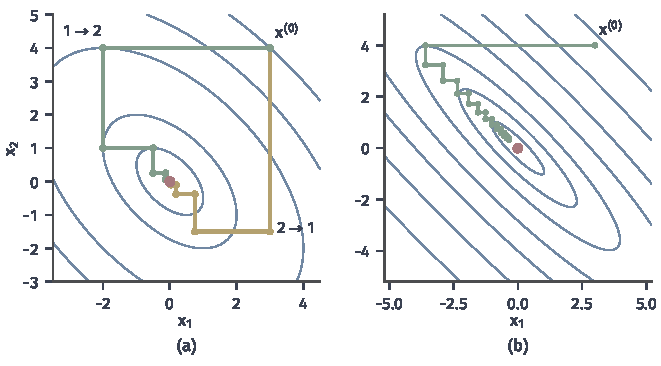
\includegraphics[width=112mm]{figures/05-optimization/04-block-optimization/matplotlib/block-cyclic-staircase/figure.pdf}
  \caption{循环坐标下降的阶梯路径，从$(3,4)$出发。(a)$c=1$，绿色先更新$x_1$，黄色先更新$x_2$，各画三轮，都按式~\eqref{eq:block-cyclic-factor}的因子$\tfrac14$收缩。(b)$c=1.8$，绿色路径画十二轮，变量耦合越强，每一阶越短。}
  \label{fig:block-cyclic-staircase}
\end{BookInlineFigure}

阶梯形状的来源是：每次只能沿坐标轴走，而谷底方向是斜的。这好比在只能走东西、南北方向的棋盘式街道上，要朝东北方向下山，只能东一段、北一段地拼出来，而且每一段都不能走得太远，否则就偏离了谷底。变量的耦合就是这条斜谷的走向，耦合越强，能走的每一段越短。

\paragraph{固定循环与每轮打乱}
二维时顺序只影响第一步，维数高了影响会大得多。实践中常在每轮开始时重新打乱顺序，这称为随机重排。它与固定循环的差别在于顺序每轮不同，与下一小节的独立随机选块的差别在于一轮内每块恰好出现一次。

后一个差别在分析中很要紧。一轮内已经选过的块不会再被选到，所以“这一步选到块$J$的概率”依赖于本轮前面选过什么，不再是与历史无关的固定值。下一小节取条件期望的论证用不上，每轮打乱的收敛分析要另外处理。

图~\ref{fig:block-order-compare}是一个数值实例。这个目标的各个变量两两等强度耦合，起点随机，固定循环明显慢于另外两种规则，每轮打乱和独立随机几乎一样。这只是一个具体问题上的观察，不是普遍定理；在另外的问题上，固定循环可以和随机规则一样快。

\begin{BookInlineFigure}
  \centering
  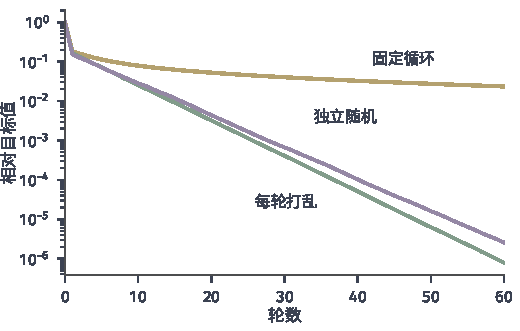
\includegraphics[width=88mm]{figures/05-optimization/04-block-optimization/matplotlib/block-order-compare/figure.pdf}
  \caption{三种更新顺序在同一目标上的比较。目标为$\tfrac12\bm{x}^\top\bm{Q}\bm{x}$，$\bm{Q}=0.1\,\bm{I}+0.9\,\bm{1}\bm{1}^\top$，$n=30$，单坐标精确更新，纵轴为目标值与起点目标值之比。黄线是固定循环，绿线是每轮打乱，紫线是独立随机（每轮$n$次更新），后两者是$30$次重复的几何平均。}
  \label{fig:block-order-compare}
\end{BookInlineFigure}

\subsection{随机块坐标下降（RBCD）}
\label{sec:block-random}

\paragraph{主要思想}
循环规则的路径取决于顺序，分析也依赖整轮的累积效应。如果每步独立地抽一块，就可以用平均值来分析单步进展，这是\term{随机块坐标下降}（randomized block coordinate descent，RBCD）的出发点。

设第$t$步与历史独立地以固定概率$p_J>0$抽取块$J$，$\sum_Jp_J=1$。记块$J$精确更新带来的真实下降量为$\Delta_J(\bm{x})=f(\bm{x})-f(\bm{x}^{+J})$，其中$\bm{x}^{+J}$是只更新块$J$得到的点。已知当前点$\bm{x}^{(t)}$时，新点的目标值是随机的，它的条件期望是各种可能结果的加权平均：
\begin{equation}
 \mathbb{E}\bigl[f(\bm{x}^{(t+1)})\mid\bm{x}^{(t)}\bigr]
 =f(\bm{x}^{(t)})-\sum_{J}p_J\,\Delta_J(\bm{x}^{(t)}).
 \label{eq:block-random-expectation}
\end{equation}
这里只用到离散情形的加权平均，条件期望的一般定义可参考\BookChapterRef{chap:conditional-expectation}{卷七第4章“条件期望与条件分布”}。

式~\eqref{eq:block-random-expectation}说明，随机规则的平均进展就是各块进展的加权平均，所以只要每块都有保底的进展，平均也有。

\paragraph{单步平均的计算}
对单坐标精确更新的二次目标，真实下降量可以写出来。条件函数是开口系数为$Q_{j,j}/2$的抛物线，当前斜率是$\partial_jf$，最小化后下降
\begin{equation}
 \Delta_j(\bm{x})=\frac{(\partial_jf(\bm{x}))^2}{2Q_{j,j}} .
 \label{eq:block-coordinate-decrease}
\end{equation}

在起点$(3,4)$，偏导数和两个下降量是
\[
 \partial_1f=10,\qquad \partial_2f=11,\qquad \Delta_1=25,\qquad \Delta_2=\frac{121}{4}=30.25 .
\]
均匀抽取时，平均下降量是
\[
 \frac12(25+30.25)=27.625,
\]
平均目标值是$37-27.625=9.375$。图~\ref{fig:block-random-average}把两个可能的结果和平均值放在一起。

\begin{BookInlineFigure}
  \centering
  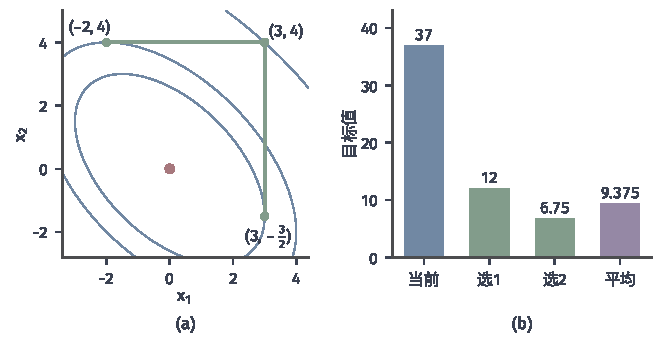
\includegraphics[width=112mm]{figures/05-optimization/04-block-optimization/matplotlib/block-random-average/figure.pdf}
  \caption{随机选块的一步。(a)从$(3,4)$出发，抽到$x_1$走到$(-2,4)$，抽到$x_2$走到$(3,-\tfrac32)$，蓝色是过这三点的等高线。(b)当前目标值、两种结果的目标值，以及均匀抽取时目标值的条件期望$9.375$（紫色）。}
  \label{fig:block-random-average}
\end{BookInlineFigure}

\paragraph{计算过程}
RBCD的计算过程与循环规则只差选块一步。例中取一个抽样结果，依次抽到块$2,1,1,2$，从$(3,4)$出发的四次更新是：
\[
 \begin{aligned}
 \text{抽到}\,2:&\quad \bm{x}=(3,\,-\tfrac32),\quad f=6.75,\\
 \text{抽到}\,1:&\quad \bm{x}=(\tfrac34,\,-\tfrac32),\quad f=1.6875,\\
 \text{抽到}\,1:&\quad \bm{x}=(\tfrac34,\,-\tfrac32),\quad f=1.6875,\\
 \text{抽到}\,2:&\quad \bm{x}=(\tfrac34,\,-\tfrac38),\quad f=0.421875 .
 \end{aligned}
\]
第三次抽到的块与上一次相同，由于上一次已经把这一块解到最优，这次更新什么也没有改变。精确块更新时连续抽到同一块就是白费，这是独立随机选块的一项代价。

\paragraph{非均匀抽取}
概率不一定要相等。比较两种选择：均匀抽取$p_j=1/n$，以及按曲率抽取$p_j=Q_{j,j}/\operatorname{tr}\bm{Q}$。后一种由式~\eqref{eq:block-coordinate-decrease}给出一个不依赖下标的平均下降：
\begin{equation}
 \sum_{j}p_j\Delta_j=\frac{\lVert\nabla f(\bm{x})\rVert_2^2}{2\operatorname{tr}\bm{Q}} .
 \label{eq:block-curvature-sampling}
\end{equation}
哪种更好取决于偏导数的分布。设$Q_{1,1}=1$，$Q_{2,2}=25$，则$p=(\tfrac1{26},\tfrac{25}{26})$。若偏导数是$(1,25)$，下降量是$(0.5,12.5)$，两种规则的平均下降量分别是$6.5$和约$12.04$，按曲率抽取更好。

若偏导数是$(3,5)$，下降量是$(4.5,0.5)$，两种规则的平均下降量分别是$2.5$和约$0.65$，按曲率抽取反而更差。所以非均匀抽取不是免费的改进，它把访问次数押在某些块上，收益要看目标的结构。

\paragraph{不能照搬逆概率校正}
“按概率抽取”很容易让人想起另一种做法：把抽到的量除以被抽中的概率，使它的期望等于要估计的量。这样做的目的是构造全梯度的无偏估计。但这里并没有估计什么：抽到块$J$时读到的偏梯度是准确的，抽样决定的只是更新哪里。

如果仍然把步长放大$1/(Bp_J)$倍，步子就会过长。例中取$p_1=\tfrac14$，放大倍数是$1/(2\cdot\tfrac14)=2$，而精确更新的位移本来是$-5$，放大后$x_1$变成
\[
 x_1=3-2\times5=-7 .
\]
新的目标值是
\[
 f(-7,4)=49-28+16=37,
\]
恰好越过最小点到了抛物线的另一侧，一点进展也没有。放大倍数再大，目标值就上升了。

因此，RBCD的速率不能从样本估计的结论推出，需要结合块内怎样求解、各块被访问的概率以及目标的结构建立。第~\ref{sec:block-convergence}小节在块内用梯度步、概率均匀的情形下给出完整的证明。

\subsection{贪心块坐标下降（Greedy BCD）}
\label{sec:block-greedy}

\paragraph{主要思想}
既然各块进展不同，为什么不直接挑进展最大的一块？这就是\term{贪心块坐标下降}（greedy block coordinate descent）。最直接的做法是对每一块都解一遍条件子问题，比较真实下降量$\Delta_J$，再选最大的。可是这等于做了$B$次块更新，只用其中一次，太浪费了。

实用的贪心规则用便宜的指标代替真实下降量。偏梯度描述当前块的陡峭程度，最简单的指标就是偏梯度的范数：
\begin{equation}
 J^{(t)}\in\argmax_{J}\ \lVert\nabla_Jf(\bm{x}^{(t)})\rVert_2 .
 \label{eq:block-gauss-southwell}
\end{equation}
这称为\term{Gauss--Southwell规则}（Gauss--Southwell rule）。在起点$(3,4)$，偏导数是$(10,11)$，规则选$x_2$，而$\Delta_2=30.25>\Delta_1=25$，确实选中了进展更大的一块。

\paragraph{块光滑常数与带曲率的指标}
偏梯度大不等于下降多：块的曲率高时，能走的距离短。要把曲率算进去，先要量化“沿一块移动时梯度变化多快”。

\begin{definition}[块光滑常数]
\label{def:block-smooth}
设$f:\mathbb{R}^n\to\mathbb{R}$可微。若存在$L_J>0$，使对一切$\bm{x}\in\mathbb{R}^n$和$\bm{h}\in\mathbb{R}^{\lvert J\rvert}$，
\begin{equation}
 \lVert\nabla_Jf(\bm{x}+\bm{U}_J\bm{h})-\nabla_Jf(\bm{x})\rVert_2\leq L_J\lVert\bm{h}\rVert_2 ,
 \label{eq:block-smooth}
\end{equation}
则称$f$关于块$J$是$L_J$光滑的，$L_J$称为\term{块光滑常数}（block smoothness constant）。
\end{definition}

固定其他块后，函数$\bm{h}\mapsto f(\bm{x}+\bm{U}_J\bm{h})$的梯度正是$\nabla_Jf(\bm{x}+\bm{U}_J\bm{h})$，式~\eqref{eq:block-smooth}说它的光滑常数是$L_J$。对这个函数用第~\ref{chap:smooth-foundations}章的下降引理，得到沿块$J$的二次上界：
\begin{equation}
 f(\bm{x}+\bm{U}_J\bm{h})\leq f(\bm{x})+\langle\nabla_Jf(\bm{x}),\bm{h}\rangle+\frac{L_J}{2}\lVert\bm{h}\rVert_2^2 .
 \label{eq:block-quadratic-upper}
\end{equation}

右边在$\bm{h}=-\nabla_Jf(\bm{x})/L_J$处取最小，代入得到一个保底的下降量：
\begin{equation}
 f(\bm{x})-f\Bigl(\bm{x}-\frac{1}{L_J}\bm{U}_J\nabla_Jf(\bm{x})\Bigr)\geq\frac{\lVert\nabla_Jf(\bm{x})\rVert_2^2}{2L_J} .
 \label{eq:block-guaranteed-decrease}
\end{equation}
于是一个更合理的指标是这个保底下降量本身，即选使$\lVert\nabla_Jf\rVert_2^2/L_J$最大的块。

举一个二者选择不同的例子。设两个坐标的偏导数是$(3,5)$，块光滑常数是$(1,25)$。按偏导数大小选$x_2$，保底下降量是$25/50=0.5$；按$\lVert\nabla_Jf\rVert_2^2/L_J$选$x_1$，保底下降量是$9/2=4.5$。

\begin{BookInlineFigure}
  \centering
  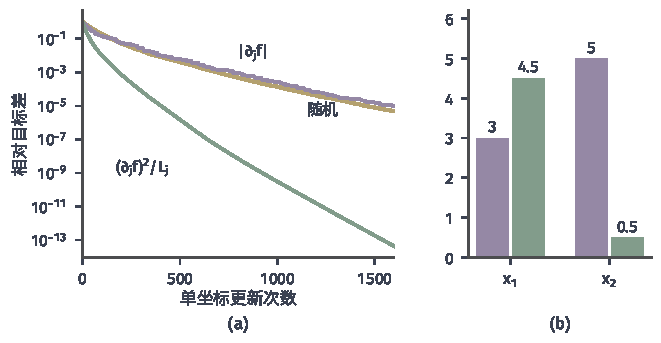
\includegraphics[width=112mm]{figures/05-optimization/04-block-optimization/matplotlib/block-greedy-rules/figure.pdf}
  \caption{选块指标的比较。(a)$N=80$、$n=40$的最小二乘，各列尺度相差很大，单坐标精确更新，纵轴为目标差与初值之比。黄线是均匀随机（$10$次重复的几何平均），紫线按$\lvert\partial_jf\rvert$选坐标，绿线按$(\partial_jf)^2/L_j$选坐标。(b)文中手算例子的两个坐标：紫色柱是$\lvert\partial_jf\rvert$，绿色柱是保底下降量$(\partial_jf)^2/(2L_j)$。}
  \label{fig:block-greedy-rules}
\end{BookInlineFigure}

图~\ref{fig:block-greedy-rules}(a)显示，当各列尺度差别很大时，只看偏梯度大小的规则并不比随机规则好，把曲率算进去之后才快了很多。(b)是手算的例子：两个指标选中了不同的坐标，而绿色柱才是能保证的下降量。

\paragraph{贪心指标的代价}
贪心规则需要知道所有块的偏梯度。若每次更新后要重算全部偏梯度，一步的代价就和一次全梯度相同，这时贪心规则很难划算。

当目标的耦合稀疏时，更新一块只影响少数几块的偏梯度，可以增量维护，并用优先队列取最大值，贪心规则才真正便宜。

\paragraph{复合目标的指标}
目标含非光滑项时，只看偏梯度会选错块。设$F=f+g$，$g(\bm{x})=\sum_Jg_J(\bm{x}_J)$是按块可分的凸函数，块$J$的二次上界加上$g_J$就成了局部模型。把模型能带来的下降量当作指标：
\begin{equation}
 \begin{aligned}
 \Delta_J^{g}(\bm{x})=-\min_{\bm{h}}\Bigl\{&\langle\nabla_Jf(\bm{x}),\bm{h}\rangle+\frac{L_J}{2}\lVert\bm{h}\rVert_2^2\\
 &+g_J(\bm{x}_J+\bm{h})-g_J(\bm{x}_J)\Bigr\}.
 \end{aligned}
 \label{eq:block-composite-index}
\end{equation}
取$g_J=\lvert\cdot\rvert$，当前$x_j=0$，$L_j=1$。若偏导数是$0.5$，$h=0$是最小点，指标为$0$，这个坐标不会动，尽管偏导数不为零。若偏导数是$2$，模型最小点是$h=-1$，指标为$0.5$，这一块才有进展可言。

\section{局部近似更新}
\label{sec:block-local}

精确块更新要求条件子问题便宜可解。许多目标不满足这一点，比如条件函数含对数或指数，每解一次都要内层迭代。这就需要回答：解不动条件子问题时，怎样在当前块上构造一个可以计算的局部模型，并用它推进完整目标？

三种模型对应三种读数。下表把它们和精确块更新放在一起比较。

\begin{BookInlineTable}
\centering
\begin{tabular}{p{20mm}p{24mm}p{22mm}p{22mm}}
\toprule
更新 & 每步读取 & 子问题 & 接受条件\\
\midrule
精确块解 & 条件函数 & 条件子问题 & 无需检验\\
BCGD & 当前点偏梯度 & 闭式的二次函数 & 步长$1/L_J$\\
APCG & 外推点偏梯度 & 闭式或邻近映射 & 无单调保证\\
块Newton & 偏梯度与块Hessian & 块内线性方程 & 线搜索等\\
\bottomrule
\end{tabular}
\end{BookInlineTable}

下面逐个看它们要解什么子问题、需要什么接受条件。

\subsection{块坐标梯度下降（BCGD）}
\label{sec:block-bcgd}

\paragraph{主要思想}
上一节的上界~\eqref{eq:block-quadratic-upper}是块$J$上的一个二次模型，它在当前点与$f$相等，并且处处不低于$f$。最小化这个上界代替最小化$f$，只走一步块梯度：
\begin{equation}
 \bm{x}_J^{(t+1)}=\bm{x}_J^{(t)}-\frac{1}{L_J}\nabla_Jf(\bm{x}^{(t)}),\qquad
 \bm{x}_i^{(t+1)}=\bm{x}_i^{(t)}\ \ (i\notin J).
 \label{eq:block-bcgd}
\end{equation}
这就是\term{块坐标梯度下降}（block coordinate gradient descent，BCGD）。由式~\eqref{eq:block-guaranteed-decrease}，每一步完整目标至少下降
\begin{equation}
 f(\bm{x}^{(t)})-f(\bm{x}^{(t+1)})\geq\frac{\lVert\nabla_Jf(\bm{x}^{(t)})\rVert_2^2}{2L_J}.
 \label{eq:block-bcgd-decrease}
\end{equation}

图~\ref{fig:block-upper-bound}(a)是一个不能闭式解出的条件函数$\varphi(z)=\sqrt{1+z^2}-z/2$，它的二阶导数不超过$1$，所以$L_J=1$。当前点$z=2$处$\varphi'(2)\approx0.394$，上界的最小点是$z^+=2-0.394=1.606$。上界（绿）紧贴在$\varphi$（蓝）的上方，上界的最小值高于真实函数在$z^+$处的值，所以真实下降量不会少于上界的下降量。

\begin{BookInlineFigure}
  \centering
  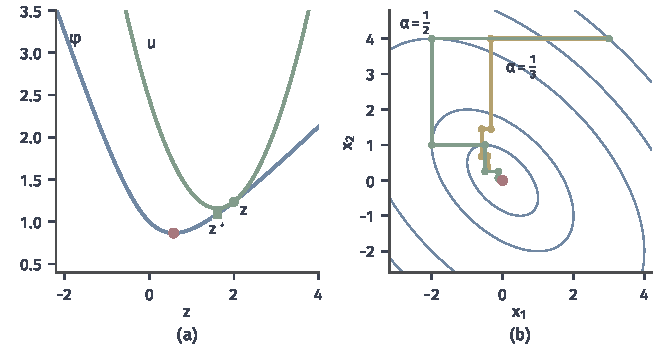
\includegraphics[width=112mm]{figures/05-optimization/04-block-optimization/matplotlib/block-upper-bound/figure.pdf}
  \caption{块梯度步的两个视角。(a)条件函数$\varphi(z)=\sqrt{1+z^2}-z/2$（蓝）与$L_J=1$的二次上界（绿），绿点是当前点$z=2$，空心点和方块分别是上界和原函数在上界最小点$z^+\approx1.606$处的值，红点是原函数的最小点$z\approx0.577$。(b)式~\eqref{eq:block-example}上循环BCGD的路径，绿色是块步长$\alpha=1/L_j=\tfrac12$，黄色是全局步长$\alpha=1/L=\tfrac13$，各画三轮。}
  \label{fig:block-upper-bound}
\end{BookInlineFigure}

\paragraph{块常数与全局常数}
最小二乘按样本数归一化时，目标是
\[
 f(\bm{x})=\frac{1}{2N}\lVert\bm{A}\bm{x}-\bm{b}\rVert_2^2 .
\]
坐标$j$的偏导数和块光滑常数是
\begin{equation}
 \partial_jf(\bm{x})=\frac{1}{N}\bm{a}_j^\top\bm{r},\qquad L_j=\frac{\lVert\bm{a}_j\rVert_2^2}{N},
 \label{eq:block-ls-constants}
\end{equation}
其中$\bm{r}=\bm{A}\bm{x}-\bm{b}$是残差。若目标不除以$N$，$L_j$和偏导数中的$1/N$同时去掉，步长与偏导数的乘积不变，所以两种写法走出的路径相同。块$J$含多列时，$L_J=\lambda_{\max}(\bm{A}_J^\top\bm{A}_J)/N$，其中$\bm{A}_J$是由这些列组成的子矩阵。

全局光滑常数是$L=\lambda_{\max}(\bm{A}^\top\bm{A})/N$。设$\bm{H}=\bm{A}^\top\bm{A}/N$半正定，每个对角元$L_j=\bm{e}_j^\top\bm{H}\bm{e}_j$不超过最大特征值，而最大特征值又不超过所有特征值之和，即迹。因此
\begin{equation}
 L_j\leq L\leq\sum_{i=1}^nL_i .
 \label{eq:block-constant-order}
\end{equation}

式~\eqref{eq:block-constant-order}的左半边解释了坐标法为什么敢走得更远：上界只要在这一个方向上成立，曲率只需按这一方向计算，而全局步长必须照顾最陡的方向。列相关性很强时$L$可接近$\sum_iL_i$，坐标步长可以比全局步长大$n$倍。

例中$\bm{A}$的两列平方范数都是$2$，未归一化时
\[
 L_1=L_2=2,\qquad L=\lambda_{\max}(\bm{Q})=3 .
\]
块步长是$\tfrac12$，全局步长是$\tfrac13$。图~\ref{fig:block-upper-bound}(b)比较了这两种步长：步长$\tfrac13$的每一阶都没有走到条件最小点，路径的收缩更慢。

\needspace{6\baselineskip}
\paragraph{变量}
\begin{itemize}
 \item $\bm{x}\in\mathbb{R}^n$：当前点。
 \item $\bm{r}=\bm{A}\bm{x}-\bm{b}\in\mathbb{R}^N$：维护的残差，读偏导数时使用。
 \item $L_j$：各坐标的块光滑常数，事先算好。
\end{itemize}

\paragraph{初始化}
算出各$L_j$和初始残差$\bm{r}^{(0)}$，令$t=0$。例中用$\bm{A}$的三行，$\bm{b}=\bm{0}$，$\bm{x}^{(0)}=(3,4)$，不除以$N$：
\[
 L_1=L_2=2,\qquad \bm{r}^{(0)}=\bm{A}\bm{x}^{(0)}=(7,3,4).
\]

\needspace{6\baselineskip}
\paragraph{每轮更新}
按某个选块规则取坐标$j$，然后：
\begin{enumerate}
 \item \textbf{读偏导数。}计算$\partial_jf=\bm{a}_j^\top\bm{r}$。例中第一轮先取$j=1$，
 \[
  \partial_1f=7+3=10 .
 \]
 \item \textbf{更新变量。}由式~\eqref{eq:block-bcgd}，位移是$\delta=-\partial_jf/L_j$，令$x_j\leftarrow x_j+\delta$。例中
 \[
  \delta=-5,\qquad x_1=-2 .
 \]
 \item \textbf{更新残差。}令$\bm{r}\leftarrow\bm{r}+\delta\bm{a}_j$，不重算矩阵乘向量。例中
 \[
  \bm{r}=(7,3,4)-5(1,1,0)=(2,-2,4).
 \]

 例中第一轮再取$j=2$，$\partial_2f=2+4=6$，$\delta=-3$，于是
 \[
  x_2=1,\qquad \bm{r}=(2,-2,4)-3(1,0,1)=(-1,-2,1).
 \]
 此时目标值是$\tfrac12\lVert\bm{r}\rVert_2^2=3$。

 例中第二轮取$j=1$，$\partial_1f=-3$，$\delta=\tfrac32$，于是
 \[
  x_1=-\tfrac12,\qquad \bm{r}=\bigl(\tfrac12,-\tfrac12,1\bigr).
 \]

 再取$j=2$，$\partial_2f=\tfrac32$，$\delta=-\tfrac34$，于是
 \[
  x_2=\tfrac14,\qquad \bm{r}=\bigl(-\tfrac14,-\tfrac12,\tfrac14\bigr).
 \]
 此时目标值是$\tfrac{3}{16}$。
\end{enumerate}

迭代结束的条件与第~\ref{sec:block-cyclic}小节相同。最终得到的点和循环精确更新完全一致，第$t$轮结束时都是$\bm{x}^{(t)}=(-2\cdot4^{1-t},4^{1-t})$。原因是二次目标的条件函数本身就是抛物线，上界~\eqref{eq:block-quadratic-upper}取$L_j=Q_{j,j}$时恰好等于条件函数，上界的最小点就是条件最小点。对一般光滑目标，两种更新不同。

\subsection{加速邻近坐标梯度（APCG）}
\label{sec:block-apcg}

\paragraph{要解决的问题}
BCGD每步只用当前点的信息，和梯度下降一样没有利用走过的路。第~\ref{chap:first-order-methods}章的加速方法靠外推把凸目标的目标差从$O(1/t)$提到$O(1/t^2)$，自然想把同样的思想用在坐标更新上。\term{加速邻近坐标梯度}（accelerated proximal coordinate gradient，APCG）方法就做这件事，并且允许目标含按块可分的非光滑项。

考虑
\begin{equation}
 \min_{\bm{x}\in\mathbb{R}^n}\ F(\bm{x})=f(\bm{x})+\sum_{J}g_J(\bm{x}_J),
 \label{eq:block-composite}
\end{equation}
其中$f$是凸函数，关于每一块满足定义~\ref{def:block-smooth}，每个$g_J$是适当、闭的凸函数。回顾第~\ref{chap:nonsmooth-composite-optimization}章的邻近映射
\[
 \operatorname{prox}_{\alpha g}(\bm{v})=\argmin_{\bm{u}}\Bigl\{g(\bm{u})+\frac{1}{2\alpha}\lVert\bm{u}-\bm{v}\rVert_2^2\Bigr\},
\]
它把“沿梯度走一步”之后的点拉回到非光滑项喜欢的位置，$g\equiv0$时就是恒等映射。

\paragraph{三条序列}
APCG维护三条序列，图~\ref{fig:block-apcg-sequences}是它们的关系。$\bm{x}^{(t)}$是报告给用户的点；$\bm{z}^{(t)}$记录累积的梯度信息，每次走较长的步子；$\bm{y}^{(t)}$是这两者的组合，只在这一点上读偏梯度。

\begin{BookInlineFigure}
  \centering
  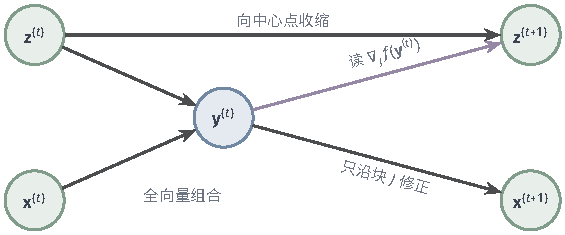
\includegraphics[width=95mm]{figures/05-optimization/04-block-optimization/tikz/block-apcg-sequences/figure.pdf}
  \caption{APCG一步中三条序列的依赖关系。$\bm{y}^{(t)}$是$\bm{x}^{(t)}$与$\bm{z}^{(t)}$的组合，这一步通常改变全部分量；在$\bm{y}^{(t)}$处读抽中块$J$的偏梯度（紫色）后，$\bm{z}$沿块$J$走一长步，$\bm{x}^{(t+1)}$只在$\bm{y}^{(t)}$的块$J$上修正一步。}
  \label{fig:block-apcg-sequences}
\end{BookInlineFigure}

为什么$\bm{z}$的步长要放大？一次只抽一块，每一块平均$B$步才轮到一次。$\bm{z}$是积累全局信息的序列，它要把偶尔读到的这一块的信息放大，才能代表整个梯度的作用，所以步长是$1/L_J$的$1/(B\alpha^{(t)})$倍。$\bm{x}$只负责走稳妥的短步。这和第~\ref{chap:first-order-methods}章的外推相似：先在外推点读梯度，再决定位移。不同的是，这里的读数只有一块，$\bm{z}$的放大倍数正是用来补偿这一点的。

分析中用到按块常数加权的范数
\begin{equation}
 \lVert\bm{x}\rVert_L^2=\sum_{J}L_J\lVert\bm{x}_J\rVert_2^2 .
 \label{eq:block-L-norm}
\end{equation}
设$f$关于这个范数有强凸常数$\mu_L\geq0$，也就是说，对任意$\bm{x},\bm{y}$，
\[
 f(\bm{y})\geq f(\bm{x})+\langle\nabla f(\bm{x}),\bm{y}-\bm{x}\rangle+\frac{\mu_L}{2}\lVert\bm{y}-\bm{x}\rVert_L^2 .
\]
$\mu_L=0$表示只要求凸。这样定义的$\mu_L$不超过$1$，因为沿块方向它受块光滑常数限制。

\paragraph{迭代公式}
记$B$为块数，选$\gamma^{(0)}\in[\mu_L,1]$且$\gamma^{(0)}>0$，令$\bm{z}^{(0)}=\bm{x}^{(0)}$。第$t$步先由下面的方程取$\alpha^{(t)}\in(0,1/B]$，并更新另外两个参数：
\begin{equation}
 \begin{gathered}
 B^2(\alpha^{(t)})^2=(1-\alpha^{(t)})\gamma^{(t)}+\alpha^{(t)}\mu_L,\\
 \gamma^{(t+1)}=B^2(\alpha^{(t)})^2,\qquad
 \beta^{(t)}=\frac{\alpha^{(t)}\mu_L}{\gamma^{(t+1)}} .
 \end{gathered}
 \label{eq:block-apcg-params}
\end{equation}
然后构造外推点和$\bm{z}$的中心点：
\begin{equation}
 \begin{aligned}
 \bm{y}^{(t)}&=\frac{\alpha^{(t)}\gamma^{(t)}\bm{z}^{(t)}+\gamma^{(t+1)}\bm{x}^{(t)}}{\alpha^{(t)}\gamma^{(t)}+\gamma^{(t+1)}},\\
 \bm{w}^{(t)}&=(1-\beta^{(t)})\bm{z}^{(t)}+\beta^{(t)}\bm{y}^{(t)} .
 \end{aligned}
 \label{eq:block-apcg-extrapolate}
\end{equation}

独立均匀地抽一块$J$，在$\bm{y}^{(t)}$处读偏梯度。记$\tau=1/(B\alpha^{(t)}L_J)$，这是比$1/L_J$更长的步长。块$J$上用邻近步更新$\bm{z}$，其余块取中心点的值：
\begin{equation}
 \bm{z}_J^{(t+1)}=\operatorname{prox}_{\tau g_J}\bigl(\bm{w}_J^{(t)}-\tau\nabla_Jf(\bm{y}^{(t)})\bigr),\qquad
 \bm{z}_i^{(t+1)}=\bm{w}_i^{(t)}\ \ (i\notin J).
 \label{eq:block-apcg-z}
\end{equation}
最后由$\bm{y}$和$\bm{z}$的变化得到新迭代点：
\begin{equation}
 \bm{x}^{(t+1)}=\bm{y}^{(t)}+B\alpha^{(t)}\bigl(\bm{z}^{(t+1)}-\bm{w}^{(t)}\bigr).
 \label{eq:block-apcg-x}
\end{equation}

式~\eqref{eq:block-apcg-z}中$\bm{z}^{(t+1)}$和$\bm{w}^{(t)}$只在块$J$上不同，所以$\bm{x}^{(t+1)}$相对$\bm{y}^{(t)}$也只改变块$J$。$g_J\equiv0$时，代入式~\eqref{eq:block-apcg-x}，块$J$上得到
\[
 \bm{x}_J^{(t+1)}=\bm{y}_J^{(t)}-\frac{1}{L_J}\nabla_Jf(\bm{y}^{(t)}),
\]
这正是在外推点上的一步BCGD。外推本身却可能改变全向量，这是加速方法计算上的主要负担，下文计入成本。

\needspace{6\baselineskip}
\paragraph{变量}
\begin{itemize}
 \item $\bm{x}^{(t)},\bm{z}^{(t)}\in\mathbb{R}^n$：报告点和累积序列。
 \item $\bm{y}^{(t)},\bm{w}^{(t)}\in\mathbb{R}^n$：外推点和$\bm{z}$的中心点，每步由前两者算出。
 \item $\alpha^{(t)},\beta^{(t)},\gamma^{(t)}$：由式~\eqref{eq:block-apcg-params}确定的标量。
\end{itemize}

\paragraph{初始化}
令$\bm{z}^{(0)}=\bm{x}^{(0)}$，选$\gamma^{(0)}$。取$\gamma^{(0)}=\mu_L>0$时，由式~\eqref{eq:block-apcg-params}可知各参数不随$t$变化：
\[
 \gamma^{(t)}=\mu_L,\qquad \alpha^{(t)}=\beta^{(t)}=\frac{\sqrt{\mu_L}}{B}.
\]

例中为了得到整齐的参数，把交叉项系数改成$c=\tfrac32$，即用$f_{3/2}$，$B=2$。此时$L_1=L_2=2$，$\lVert\bm{x}\rVert_L^2=2\lVert\bm{x}\rVert_2^2$，Hessian的最小特征值是$\tfrac12$，于是
\[
 \mu_L=\frac14,\qquad \alpha^{(t)}=\beta^{(t)}=\frac14 .
\]
起点仍取$\bm{x}^{(0)}=\bm{z}^{(0)}=(3,4)$，目标值$f=43$。$g_J\equiv0$，步长$\tau=1/(2\cdot\tfrac14\cdot2)=1$。

\needspace{6\baselineskip}
\paragraph{每轮更新}
第$t$步依次做：
\begin{enumerate}
 \item \textbf{外推。}按式~\eqref{eq:block-apcg-extrapolate}算$\bm{y}^{(t)}$和$\bm{w}^{(t)}$。例中公式化为
 \[
  \bm{y}=\frac{4\bm{x}+\bm{z}}{5},\qquad \bm{w}=\frac34\bm{z}+\frac14\bm{y}.
 \]
 第一步$\bm{x}=\bm{z}$，所以$\bm{y}=\bm{w}=(3,4)$。
 \item \textbf{抽块并读偏梯度。}例中第一步设抽到块$1$，
 \[
  \partial_1f(\bm{y})=2\cdot3+\tfrac32\cdot4=12 .
 \]
 \item \textbf{更新$\bm{z}$。}按式~\eqref{eq:block-apcg-z}。例中$\tau=1$，块$J$上$\bm{z}_J^{+}=\bm{w}_J-\nabla_Jf(\bm{y})$，第一步
 \[
  \bm{z}^{(1)}=(-9,4).
 \]
 \item \textbf{更新$\bm{x}$。}按式~\eqref{eq:block-apcg-x}。例中块$J$上$\bm{x}_J^{+}=\bm{y}_J-\tfrac12\nabla_Jf(\bm{y})$，第一步
 \[
  \bm{x}^{(1)}=(-3,4),\qquad f(\bm{x}^{(1)})=7 .
 \]

 例中第二步设抽到块$2$。先算外推点和中心点，
 \[
  \bm{y}=(-4.2,\,4),\qquad \bm{w}=(-7.8,\,4).
 \]
 偏导数$\partial_2f(\bm{y})=\tfrac32(-4.2)+8=1.7$，于是
 \[
  \bm{z}^{(2)}=(-7.8,\,2.3),\qquad \bm{x}^{(2)}=(-4.2,\,3.15),\qquad f(\bm{x}^{(2)})=7.7175 .
 \]

 例中第三步设抽到块$1$，同样计算得
 \[
  \bm{y}=(-4.92,\,2.98),\qquad \bm{w}=(-7.08,\,2.47),\qquad \partial_1f(\bm{y})=-5.37 ,
 \]
 于是
 \[
  \bm{z}^{(3)}=(-1.71,\,2.47),\qquad \bm{x}^{(3)}=(-2.235,\,2.98),\qquad f(\bm{x}^{(3)})=3.885175 .
 \]
\end{enumerate}

第二步的目标值从$7$升到了$7.7175$，这不是计算错误。APCG在外推点上读偏梯度，$\bm{x}^{(t+1)}$相对$\bm{y}^{(t)}$有下降保证，相对$\bm{x}^{(t)}$却没有，目标值不是单调的。迭代持续到外部设定的更新次数或目标差估计达到要求为止，图~\ref{fig:block-apcg-rate}(b)是继续迭代的结果。

\paragraph{收敛结论}
下面的结论把成立所需的条件都列了出来。证明要构造随机的估计序列，并逐步跟踪参数$\alpha^{(t)},\gamma^{(t)}$的递推，篇幅较长，读者可查阅Lin、Lu和Xiao关于APCG方法的原始论文。

\begin{theorem}[APCG的收敛率]
\label{thm:block-apcg}
设问题~\eqref{eq:block-composite}的解集非空，$f$是凸函数，满足定义~\ref{def:block-smooth}（全空间上成立），且关于范数~\eqref{eq:block-L-norm}的强凸常数为$\mu_L\geq0$；每个$g_J$是适当、闭的凸函数，邻近子问题~\eqref{eq:block-apcg-z}精确求解。设每步独立均匀地抽块，参数按式~\eqref{eq:block-apcg-params}取，$\gamma^{(0)}\in[\mu_L,1]$，$\gamma^{(0)}>0$。记$R_0=\min\lVert\bm{x}^{(0)}-\bm{x}^\star\rVert_L$，最小值取遍所有最优解。则对一切$t\geq0$，
\begin{equation}
 \mathbb{E}\bigl[F(\bm{x}^{(t)})\bigr]-F^\star\leq
 \min\Bigl\{\Bigl(1-\frac{\sqrt{\mu_L}}{B}\Bigr)^{t},\ \Bigl(\frac{2B}{2B+t\sqrt{\gamma^{(0)}}}\Bigr)^{2}\Bigr\}\,E_0,
 \label{eq:block-apcg-rate}
\end{equation}
其中
\begin{equation}
 E_0=F(\bm{x}^{(0)})-F^\star+\frac{\gamma^{(0)}}{2}R_0^2 .
 \label{eq:block-apcg-e0}
\end{equation}
\end{theorem}

这个结论有三层含义。$\mu_L=0$时，第二项给出$O(B^2/t^2)$的期望目标差，$t$次更新相当于$t/B$轮，所以按轮数算是$O(1/(t/B)^2)$，这是加速率。$\mu_L>0$且取$\gamma^{(0)}=\mu_L$时，第一项给出线性率，因子是$1-\sqrt{\mu_L}/B$，而第~\ref{sec:block-convergence}小节的BCGD因子相当于$1-\mu_L/B$，根号带来的差别在$\mu_L$很小时才明显。

例中$\mu_L=\tfrac14$，$B=2$，所以APCG的因子是$1-\tfrac14=\tfrac34$，BCGD的因子是$1-\tfrac18=\tfrac78$。定理保证的都是期望，并要求块是独立均匀抽取的，单次运行的路径可能波动。

条件的作用值得逐条看。块光滑常数给出沿块的二次上界，步长由它决定；精确的块邻近求解让加速递推的不等式能闭合，若解得不准，误差会在递推中累积，第~\ref{sec:block-inexact}小节讨论的误差控制不能直接搬过来；解的存在保证$R_0$有限，否则右端没有意义。

图~\ref{fig:block-apcg-rate}显示了加速的效果和代价。(a)是链式二次目标，没有可用的强凸常数，APCG（绿）的目标差贴着虚线$t^{-2}$下降，明显快于BCGD（黄）。(b)是手算例子的延续，APCG整体更快，但曲线有回升。

\begin{BookInlineFigure}
  \centering
  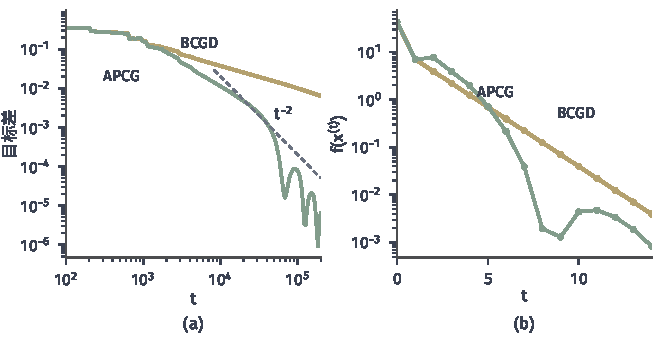
\includegraphics[width=112mm]{figures/05-optimization/04-block-optimization/matplotlib/block-apcg-rate/figure.pdf}
  \caption{APCG的数值表现。(a)链式二次目标，$n=200$，单坐标块，绿线是APCG（$\mu_L=0$），黄线是BCGD，都是$4$次独立运行的平均，灰色虚线是斜率为$-2$的参考线。(b)$f_{3/2}$从$(3,4)$出发，按块$1,2,1,2,\ldots$的顺序，绿线是APCG（$\alpha^{(t)}=\beta^{(t)}=\tfrac14$），黄线是步长$\tfrac12$的BCGD，APCG的目标值并不单调。}
  \label{fig:block-apcg-rate}
\end{BookInlineFigure}

\paragraph{计算成本}
一步APCG除了读一个偏梯度，还要做式~\eqref{eq:block-apcg-extrapolate}这样的全向量组合，直接实现的代价是$O(n)$，可能抵消单坐标更新省下的计算。实现时可以把$\bm{x},\bm{z}$写成两个基向量的线性组合，组合系数是标量，每步只更新基向量的一块，外推就不必真正展开。

偏梯度读取仍然需要在$\bm{y}^{(t)}$处求值。对最小二乘，维护$\bm{A}$作用在两个基向量上的结果即可，每步成本和BCGD同量级。这一点依赖目标的结构；$\nabla_Jf$不能增量维护时，一步的成本仍是$O(n)$或更高。

\subsection{块坐标Newton法}
\label{sec:block-newton}

\paragraph{主要思想}
块梯度步只用一阶信息，块内变量强耦合时，它和全局梯度下降一样走折线。第~\ref{chap:second-order-methods}章用Hessian修正方向，这里只对当前块做同样的事。设$f$二阶连续可微，把二阶Taylor模型限制在块$J$上：
\[
 m_J(\bm{h})=f(\bm{x})+\langle\nabla_Jf(\bm{x}),\bm{h}\rangle+\frac12\bm{h}^\top\bm{H}_{J,J}\bm{h},
\]
其中$\bm{H}_{J,J}$是Hessian的块$J$主子矩阵，即
\[
 \bm{H}_{J,J}=\bm{U}_J^\top\nabla^2f(\bm{x})\bm{U}_J .
\]
$\bm{H}_{J,J}$正定时模型有唯一最小点，得到块Newton方向：
\begin{equation}
 \bm{d}_J=-\bm{H}_{J,J}^{-1}\nabla_Jf(\bm{x}).
 \label{eq:block-newton}
\end{equation}
\term{块坐标Newton法}（block coordinate Newton method）沿这个方向更新块$J$，其余块不动。

\paragraph{正定性、修正与阻尼}
第~\ref{chap:second-order-methods}章对完整Newton法提出的三个问题，在这里同样存在，只是规模换成了块。第一是正定性：若$\nabla^2f(\bm{x})$正定，它的任何主子矩阵也正定，并且最小特征值不小于$\nabla^2f(\bm{x})$的最小特征值，块方向总是下降方向。

非凸目标的$\bm{H}_{J,J}$可能不定，这时要加修正，比如把它换成$\bm{H}_{J,J}+\tau\bm{I}$。第二是步长：二阶模型只是局部近似，不保证$\bm{d}_J$上目标下降，需要沿该方向回溯，令$\bm{x}_J^{+}=\bm{x}_J+\alpha\bm{d}_J$，用完整目标检验$\alpha$是否可接受。第三是成本：下面单独计算。

\paragraph{何时等于精确块解}
二次目标的$\bm{H}_{J,J}$是常数$\bm{Q}_{J,J}$，二阶模型恰好等于条件函数。令$\bm{d}_J$由式~\eqref{eq:block-newton}给出，$\bm{x}_J+\bm{d}_J$就是式~\eqref{eq:block-quadratic-solve}的精确块解。

例中$J=\{1\}$，点$(3,4)$处$\partial_1f=10$，$H_{1,1}=2$，方向$d_1=-5$，新值$x_1=-2$，和精确块解相同。

一般的非线性目标则不同。设条件函数是$\varphi(z)=z^4+2z$，当前$z=1$，则
\[
 \varphi'(1)=6,\qquad\varphi''(1)=12,\qquad z^{+}=1-\frac{6}{12}=0.5 .
\]
而精确块解满足$4z^3+2=0$，即$z\approx-0.794$，两者差很远。Newton步解的是模型，只有模型足够准确时才接近精确块解。图~\ref{fig:block-newton-slice}对比了这两种情形。

\begin{BookInlineFigure}
  \centering
  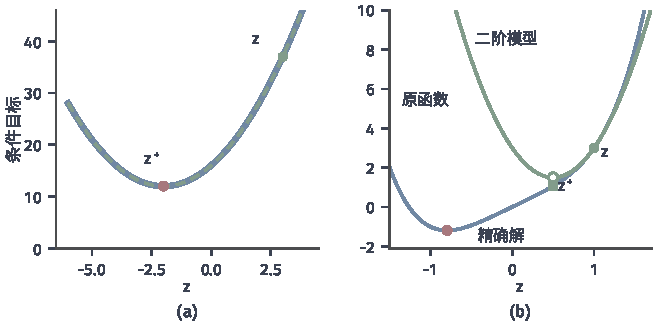
\includegraphics[width=112mm]{figures/05-optimization/04-block-optimization/matplotlib/block-newton-slice/figure.pdf}
  \caption{块Newton步与精确块解。(a)二次条件函数$\varphi(z)=z^2+4z+16$，蓝色实线与绿色虚线分别是原函数和二阶模型，两者重合，Newton步一步到达条件最小点。(b)非二次条件函数$\varphi(z)=z^4+2z$在$z=1$处，绿色的二阶模型只在附近贴近原函数（蓝），它的最小点$z^+=0.5$（空心点）与原函数的最小点（红）相距较远。}
  \label{fig:block-newton-slice}
\end{BookInlineFigure}

\paragraph{成本}
块大小$p=\lvert J\rvert$时，一步块Newton需要形成$\bm{H}_{J,J}$的$O(p^2)$个元素，并以约$p^3/3$的运算量做Cholesky分解。固定其他块时若$\bm{H}_{J,J}$不变，分解可以复用，这在二次目标上正是图~\ref{fig:block-size-cost}的成本模型；一般非线性目标的Hessian随迭代变化，分解要反复计算。

\section{交替极小化}
\label{sec:block-alternating}

前面的块多半是单个坐标或一小组坐标。有些问题的变量天然分成少数几组，每组固定其余后都容易解。沿用精确块更新依次解这几组，能得到什么，又在哪里止步？

\term{交替极小化}（alternating minimization）就是块数较少时的精确BCD，它是组织条件求解的一种方式，并不是一类新的优化理论。下面以矩阵分解为主例，并区分三个常被混在一起的性质。分别凸使每个条件子问题容易解；块解唯一使迭代有确定含义，并支撑极限分析；联合凸才能把驻点推到全局最优。

\subsection{交替最小二乘（ALS）}
\label{sec:block-als}

\paragraph{主要思想}
回到矩阵分解问题
\begin{equation}
 \min_{\bm{U},\bm{V}}\ \Phi(\bm{U},\bm{V})=\lVert\bm{Y}-\bm{U}\bm{V}^\top\rVert_F^2 .
 \label{eq:block-factorization}
\end{equation}
它关于$(\bm{U},\bm{V})$联合起来不是凸函数，但固定一个因子，另一个因子就是线性最小二乘。\term{交替最小二乘}（alternating least squares，ALS）轮流解这两个问题。

固定$\bm{V}$，目标按行拆开。记$\bm{Y}$的第$i$行为$\bm{y}_i^\top$，$\bm{U}$的第$i$行为$\bm{u}_i^\top$，则
\[
 \lVert\bm{Y}-\bm{U}\bm{V}^\top\rVert_F^2=\sum_{i=1}^{p}\lVert\bm{y}_i-\bm{V}\bm{u}_i\rVert_2^2 .
\]
每一行都是一个系数矩阵为$\bm{V}$的最小二乘问题，图~\ref{fig:block-als-structure}(a)标出了这种按行的结构。

\begin{BookInlineFigure}
  \centering
  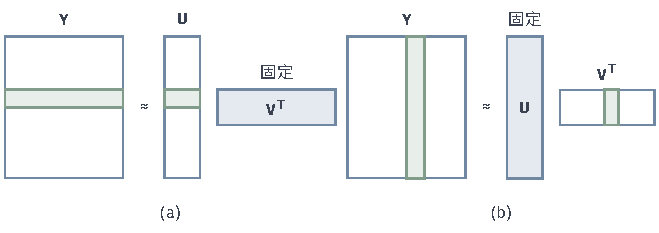
\includegraphics[width=110mm]{figures/05-optimization/04-block-optimization/tikz/block-als-structure/figure.pdf}
  \caption{ALS的两个半步。(a)固定$\bm{V}^\top$（蓝）时，$\bm{Y}$的每一行只依赖$\bm{U}$的对应行（绿），问题拆成$p$个共用系数矩阵的最小二乘。(b)固定$\bm{U}$（蓝）时，$\bm{Y}$的每一列只依赖$\bm{V}^\top$的对应列，同样拆开。}
  \label{fig:block-als-structure}
\end{BookInlineFigure}

对$\bm{u}_i$求导并把$p$行合起来，得到正规方程
\[
 \bm{U}\bm{V}^\top\bm{V}=\bm{Y}\bm{V}.
\]
若$\bm{V}$满列秩，$\bm{V}^\top\bm{V}$可逆，解唯一：
\begin{equation}
 \bm{U}^{+}=\bm{Y}\bm{V}(\bm{V}^\top\bm{V})^{-1}.
 \label{eq:block-als-u}
\end{equation}
同理，固定$\bm{U}$且$\bm{U}$满列秩时，
\begin{equation}
 \bm{V}^{+}=\bm{Y}^\top\bm{U}(\bm{U}^\top\bm{U})^{-1}.
 \label{eq:block-als-v}
\end{equation}

\paragraph{秩亏时的选解}
若$\bm{V}$不满列秩，正规方程有无穷多解。此时要规定选哪一个，常用的是Frobenius范数最小的解
\[
 \bm{U}^{+}=\bm{Y}\bm{V}(\bm{V}^\top\bm{V})^{\dagger},
\]
其中$\dagger$表示伪逆。比如$\bm{V}=\bm{0}$时，任何$\bm{U}$都使目标等于$\lVert\bm{Y}\rVert_F^2$，这个规则选$\bm{U}=\bm{0}$。

\paragraph{三种计算方式}
式~\eqref{eq:block-als-u}要解的是$p$个右端不同、系数相同的方程。系数矩阵是同一个，逐行重新分解是浪费，分解只需做一次。设$\bm{V}\in\mathbb{R}^{q\times r}$，$\bm{Y}$稠密，一个半步的主要运算是：
\begin{itemize}
 \item 形成$\bm{V}^\top\bm{V}$，约$qr^2$；形成$\bm{Y}\bm{V}$，约$pqr$。
 \item 做一次Cholesky分解，约$r^3/3$。
 \item 对$p$行各做一次前代回代，约$2pr^2$。
\end{itemize}
$\bm{Y}$稀疏时第二项换成$r$乘以非零元数。分解的条件数是$\bm{V}$的条件数的平方，$\bm{V}$接近秩亏时，改用$\bm{V}$的QR分解更稳定，但一次分解的运算量约为$2qr^2$。

加入正则项$\gamma(\lVert\bm{U}\rVert_F^2+\lVert\bm{V}\rVert_F^2)$，$\gamma>0$，后，系数矩阵变成严格正定，子问题总有唯一解：
\begin{equation}
 \bm{U}^{+}=\bm{Y}\bm{V}(\bm{V}^\top\bm{V}+\gamma\bm{I})^{-1}.
 \label{eq:block-als-ridge}
\end{equation}
秩亏的麻烦由此消除，代价是目标改变了，解被拉向零。

\paragraph{完整目标不增}
两个半步各是一次精确块更新，由引理~\ref{lem:block-exact-descent}，连起来就是
\begin{equation}
 \Phi(\bm{U}^{(t+1)},\bm{V}^{(t+1)})\leq\Phi(\bm{U}^{(t+1)},\bm{V}^{(t)})\leq\Phi(\bm{U}^{(t)},\bm{V}^{(t)}).
 \label{eq:block-als-monotone}
\end{equation}
目标有下界$0$，目标值序列因此收敛。注意这只说明目标值收敛，并不说明因子本身收敛，因为$(c\bm{U},\bm{V}/c)$与$(\bm{U},\bm{V})$有相同的目标值，因子的尺度不由目标决定。

\needspace{6\baselineskip}
\paragraph{变量}
\begin{itemize}
 \item $\bm{U}\in\mathbb{R}^{p\times r}$，$\bm{V}\in\mathbb{R}^{q\times r}$：两个因子。
 \item $\bm{Y}\in\mathbb{R}^{p\times q}$：数据矩阵，只读。
\end{itemize}

\paragraph{初始化}
选定秩$r$，随机初始化$\bm{V}^{(0)}$。下面用一个$r=1$的例子，因子都是向量，记为$\bm{u},\bm{v}$：
\[
 \bm{Y}=\begin{bmatrix}3&1\\1&3\end{bmatrix},\qquad \bm{v}^{(0)}=(1,0),
\]
于是$\lVert\bm{Y}\rVert_F^2=20$。

\needspace{6\baselineskip}
\paragraph{每轮更新}
在第$t$轮：
\begin{enumerate}
 \item \textbf{更新$\bm{U}$。}由式~\eqref{eq:block-als-u}计算。例中$\bm{u}=\bm{Y}\bm{v}/\lVert\bm{v}\rVert_2^2$，第一轮
 \[
  \bm{u}^{(1)}=(3,1),\qquad \Phi=10 .
 \]
 \item \textbf{更新$\bm{V}$。}由式~\eqref{eq:block-als-v}计算。例中$\bm{v}=\bm{Y}^\top\bm{u}/\lVert\bm{u}\rVert_2^2$，第一轮
 \[
  \bm{v}^{(1)}=\frac{(10,6)}{10}=(1,0.6),\qquad \Phi=6.4 .
 \]

 第二轮用$\bm{v}^{(1)}$计算，$\lVert\bm{v}^{(1)}\rVert_2^2=1.36$，于是
 \[
  \bm{u}^{(2)}=\frac{(3.6,2.8)}{1.36}\approx(2.647,2.059),\qquad \Phi\approx4.706 .
 \]
 再更新$\bm{v}$，$\lVert\bm{u}^{(2)}\rVert_2^2\approx11.246$，于是
 \[
  \bm{v}^{(2)}\approx(0.889,0.785),\qquad \Phi\approx4.185 .
 \]
 \item \textbf{检查停止。}目标值的相对下降或因子的相对变化小于容差时结束。
\end{enumerate}

第二轮的$\bm{v}$两个分量之比已经接近$1$，最终得到$\bm{u},\bm{v}$都平行于$(1,1)$，目标值趋于$4$。这个$4$正是$\bm{Y}$的第二个奇异值的平方，由矩阵逼近的结论，它是所有秩$1$逼近的最小误差；相关的定理可参考\BookChapterRef{chap:matrix-approximation}{卷二第18章“矩阵逼近”}。

这个例子中，交替更新实际上是幂迭代。把两个半步合起来，$\bm{v}$的新方向正比于$\bm{Y}^\top\bm{Y}\bm{v}$，$\bm{Y}^\top\bm{Y}$的特征值是$16$和$4$，所以偏离主方向的分量每轮缩小到$\tfrac14$。

图~\ref{fig:block-als-descent}(a)是这个例子的目标值阶梯，(b)取一个噪声较大的$40\times25$矩阵，从不同的随机起点出发，都很快接近截断奇异值分解给出的最优值。一般情形下ALS并不总能这样达到全局最优，下一小节就是反例。

\begin{BookInlineFigure}
  \centering
  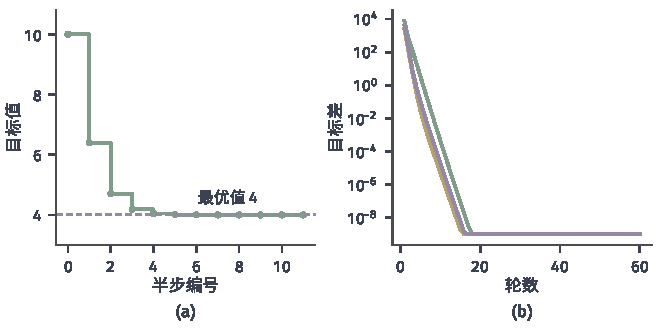
\includegraphics[width=112mm]{figures/05-optimization/04-block-optimization/matplotlib/block-als-descent/figure.pdf}
  \caption{ALS的目标值。(a)文中$2\times2$的例子，每半步记录一次，绿色阶梯单调下降，紫色虚线是最优秩$1$误差$4$。(b)$40\times25$的矩阵（秩$3$信号加噪声），$r=3$，三种颜色是三个随机起点，纵轴是目标值与截断奇异值分解最优值之差，下方平台是绘图的截断值。}
  \label{fig:block-als-descent}
\end{BookInlineFigure}

\subsection{逐块最优的局限}
\label{sec:block-limits}

\paragraph{停在鞍点的例子}
每一步都精确解出了条件子问题，最后能到全局最优吗？考虑带正则的双线性目标，$0<\rho<1$：
\begin{equation}
 \Phi_\rho(u,v)=\frac12(uv-1)^2+\frac{\rho}{2}(u^2+v^2).
 \label{eq:block-saddle-example}
\end{equation}
固定$v$，它是$u$的二次函数，$u^2$的系数是$(v^2+\rho)/2>0$，所以条件子问题有唯一解。令偏导数为零，得到
\begin{equation}
 u=\frac{v}{v^2+\rho},\qquad v=\frac{u}{u^2+\rho}.
 \label{eq:block-saddle-update}
\end{equation}
这里两个条件子问题都严格凸、解唯一，看上去已经是最好的情形了。

下面取$\rho=0.36$。全局最小点在$u=v=\pm\sqrt{1-\rho}=\pm0.8$，最小值是$\rho-\rho^2/2=0.2952$。从$v=0.6$出发，迭代是
\[
 u=0.8333,\quad v=0.7903,\quad u=0.8027,\quad v=0.7992,\quad u=0.8002,
\]
目标值从$0.3148$很快降到最小值附近。

现在换一个起点：$u=v=0$。由式~\eqref{eq:block-saddle-update}，两个更新都给出$0$，迭代永远停在原点，目标值是$\tfrac12$。

原点是什么样的点？两个偏导数都是$0$，它是驻点。它的Hessian是
\[
 \begin{bmatrix}\rho&-1\\-1&\rho\end{bmatrix},
\]
特征值$\rho-1=-0.64$和$\rho+1=1.36$一负一正，所以原点是鞍点，不是极小点。图~\ref{fig:block-saddle}画出了这一点。

\begin{BookInlineFigure}
  \centering
  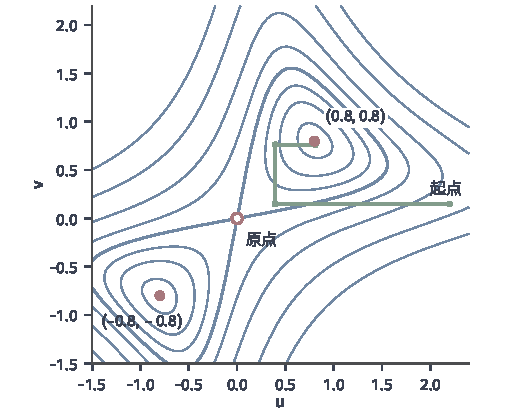
\includegraphics[width=88mm]{figures/05-optimization/04-block-optimization/matplotlib/block-saddle/figure.pdf}
  \caption{交替极小化与鞍点。$\Phi_\rho$的等高线（$\rho=0.36$），加粗的一条是$\Phi_\rho=\tfrac12$，正好穿过原点。绿色折线从$(2.2,0.15)$出发，收敛到红点$(0.8,0.8)$。红色空心点是原点：两个条件子问题的解都是$0$，从这里出发的迭代不动，而沿Hessian的负特征方向目标还能下降。}
  \label{fig:block-saddle}
\end{BookInlineFigure}

原点并不吸引路径。在原点附近$u\approx v/\rho$，$v\approx u/\rho$，一轮下来$v$约放大$1/\rho^2\approx7.7$倍，所以只要$v$不恰好为零，迭代就会被推开。图中的绿线就从靠近原点的横线上逃开了。不过这种稳定性分析需要另外的工作，逐块最优这个性质本身不能排除鞍点。

\paragraph{三个层次的对比}
再把第~\ref{sec:block-coupling}小节的反例放进来，就能看清三个不同的层次。下表中，“逐块最优”指对每个块，当前点都是条件子问题的最优解。

\begin{BookInlineTable}
\centering
\begin{tabular}{lll}
\toprule
情形 & 逐块最优 $\Rightarrow$ 驻点？ & 驻点 $\Rightarrow$ 全局最优？\\
\midrule
光滑非凸（例~\eqref{eq:block-saddle-example}） & 是 & 否，原点是鞍点\\
不可分（例~\eqref{eq:block-nonsmooth-example}） & 否，原点不是驻点 & 凸时为是\\
光滑加可分凸项，联合凸 & 是 & 是\\
\bottomrule
\end{tabular}
\end{BookInlineTable}

第一列的结论：对光滑目标，每个块的偏梯度为零，合起来就是整个梯度为零，所以逐块最优蕴含驻点。可分的非光滑项也可以这样合起来。不可分的非光滑项不行，这正是例~\eqref{eq:block-nonsmooth-example}停滞的原因。

第二列的结论：驻点推出全局最优需要联合凸性，只是分别凸还不够。在例~\eqref{eq:block-saddle-example}中，固定任一变量时函数都凸，联合起来却不凸。

\paragraph{联合凸时的结论}
联合凸性加上可分结构后，上述三个层次重合，这时逐块最优就是全局最优。

\begin{lemma}[联合凸时逐块最优即全局最优]
\label{lem:block-joint-convex}
设$F=f+\sum_Jg_J$，$f$在$\mathbb{R}^n$上凸且可微，各$g_J$是适当凸函数。若$\bar{\bm{x}}$满足$F(\bar{\bm{x}})<+\infty$，且对每个块$J$，$\bar{\bm{x}}_J$是块$J$条件子问题的最优解，则$\bar{\bm{x}}$是$F$的全局最小点。
\end{lemma}

\begin{proof}
取任意$\bm{y}\in\mathbb{R}^n$，固定一块$J$，令$\bm{h}=\bm{y}_J-\bar{\bm{x}}_J$。对$s\in(0,1]$，由块最优性，
\[
 f(\bar{\bm{x}}+s\bm{U}_J\bm{h})+g_J(\bar{\bm{x}}_J+s\bm{h})\geq f(\bar{\bm{x}})+g_J(\bar{\bm{x}}_J).
\]

由$g_J$的凸性，
\[
 g_J(\bar{\bm{x}}_J+s\bm{h})\leq(1-s)g_J(\bar{\bm{x}}_J)+sg_J(\bm{y}_J),
\]
代入并整理得
\[
 \frac{f(\bar{\bm{x}}+s\bm{U}_J\bm{h})-f(\bar{\bm{x}})}{s}+g_J(\bm{y}_J)-g_J(\bar{\bm{x}}_J)\geq0 .
\]
令$s\downarrow0$，第一项趋于$\langle\nabla_Jf(\bar{\bm{x}}),\bm{h}\rangle$，于是
\[
 \langle\nabla_Jf(\bar{\bm{x}}),\bm{y}_J-\bar{\bm{x}}_J\rangle+g_J(\bm{y}_J)-g_J(\bar{\bm{x}}_J)\geq0 .
\]

对所有块求和。$f$是凸函数，所以
\[
 f(\bm{y})\geq f(\bar{\bm{x}})+\langle\nabla f(\bar{\bm{x}}),\bm{y}-\bar{\bm{x}}\rangle,
\]
于是
\[
 \begin{aligned}
 F(\bm{y})-F(\bar{\bm{x}})
 &\geq\langle\nabla f(\bar{\bm{x}}),\bm{y}-\bar{\bm{x}}\rangle+\sum_J\bigl(g_J(\bm{y}_J)-g_J(\bar{\bm{x}}_J)\bigr)\\
 &\geq0 .
 \end{aligned}
\]
\end{proof}

证明中用到可分结构的地方是把各块的不等式相加。这正好解释了例~\eqref{eq:block-nonsmooth-example}为什么失败：它的非光滑项不能写成$\sum_Jg_J(\bm{x}_J)$，两块的不等式加不到一起。

\section{块上界最小化（BSUM）}
\label{sec:block-bsum}

前面几种更新（精确块解、块梯度步）看起来不同，下降的理由却相似：都在当前块上最小化一个不低于原目标、在当前点贴住原目标的函数。于是要问：这样的函数需要满足什么条件，才能保证完整目标的进展？

第~\ref{chap:nonsmooth-composite-optimization}章的MM方法对全部变量最小化上界，\term{块上界最小化}（block successive upper-bound minimization，BSUM）把同样的想法用在块上。它研究的是代理模型的构造和保证，可以覆盖好几种前面的更新，并不限于精确交替求解。

\subsection{块上界的条件}
\label{sec:block-bsum-conditions}

\paragraph{框架}
设$F:\bm{C}\to\mathbb{R}$，$\bm{C}$是闭凸集的乘积~\eqref{eq:block-product-set}。对每个块$J$和当前点$\bm{y}\in\bm{C}$，取一个定义在$\bm{C}_J$上的函数$u_J(\cdot;\bm{y})$，每次选块$J$后最小化它：
\begin{equation}
 \bm{x}_J^{(t+1)}\in\argmin_{\bm{z}\in\bm{C}_J}u_J(\bm{z};\bm{x}^{(t)}),\qquad
 \bm{x}_i^{(t+1)}=\bm{x}_i^{(t)}\ \ (i\notin J).
 \label{eq:block-bsum}
\end{equation}
直观地说，这是在目标上方扣一只贴住当前点的碗。碗不低于目标，碗底不高于当前点，所以从碗底的位置看，目标一定没有升高。好的$u_J$既要比条件函数容易最小化，又要真正起到这只碗的作用。下面的定义列出了所需的条件。

\begin{definition}[块上界]
\label{def:block-upper-bound}
称$u_J$是块$J$的\term{块上界}（block upper bound），如果对一切$\bm{y}\in\bm{C}$和$\bm{z}\in\bm{C}_J$，以及一切满足$\bm{y}_J+\bm{d}\in\bm{C}_J$的方向$\bm{d}$，下列条件成立：
\begin{align}
 u_J(\bm{y}_J;\bm{y})&=F(\bm{y}),\label{eq:block-ub-equal}\\
 u_J(\bm{z};\bm{y})&\geq F\bigl(\bm{y}+\bm{U}_J(\bm{z}-\bm{y}_J)\bigr),\label{eq:block-ub-upper}\\
 u_J'(\bm{y}_J;\bm{y};\bm{d})&=F'(\bm{y};\bm{U}_J\bm{d}),\label{eq:block-ub-derivative}
\end{align}
其中左端的方向导数对第一个变量取，且$u_J$关于$(\bm{z},\bm{y})$连续。
\end{definition}

\paragraph{条件的作用}
式~\eqref{eq:block-ub-upper}是上界条件，式~\eqref{eq:block-ub-equal}是当前点相等的条件，两者合起来给出下降：
\begin{equation}
 F(\bm{x}^{(t+1)})\leq u_J(\bm{x}_J^{(t+1)};\bm{x}^{(t)})\leq u_J(\bm{x}_J^{(t)};\bm{x}^{(t)})=F(\bm{x}^{(t)}).
 \label{eq:block-bsum-descent}
\end{equation}
第一个不等号用上界，第二个不等号用$\bm{x}_J^{(t+1)}$是最小点，等号用当前点相等。

一阶条件~\eqref{eq:block-ub-derivative}不是用来保证下降的，而是让停下来的点有意义。如果迭代在$\bm{y}_J$不动，说明$\bm{y}_J$最小化了$u_J$，那么$u_J$在$\bm{y}_J$的方向导数非负；有了一阶条件，$F$沿块方向的方向导数也非负。连续性则让这些性质能够传到极限点。

\paragraph{去掉条件会怎样}
图~\ref{fig:block-bsum-conditions}用同一个条件函数说明。当前点是$z=2$。(a)是合格的二次上界。

(b)是二阶Taylor模型，曲率取真实值$\varphi''(2)\approx0.089$。它不是上界，最小点在$z\approx-2.41$，模型预测目标值大幅下降，实际$\varphi(-2.41)\approx3.81$却远高于当前值$1.24$。上界条件被破坏，下降链断了。

(c)是上界$\varphi(2)+1.5\lvert z-2\rvert$。因为$\lvert\varphi'\rvert\leq1.5$，它确实是上界，并且在当前点相等，于是满足前两个条件。但它在$z=2$处有尖角，最小点就是当前点，算法不动，而$\varphi'(2)\neq0$。这说明缺了一阶条件，下降虽然仍然成立，却可以停在任何点上。

\begin{BookInlineFigure}
  \centering
  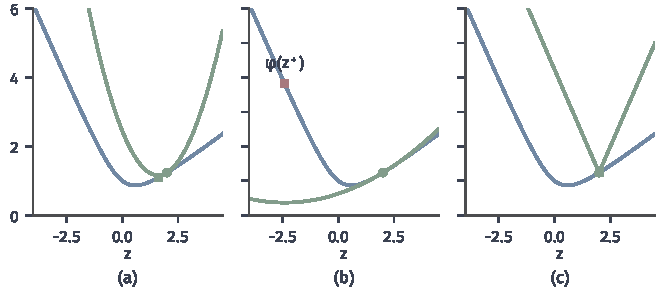
\includegraphics[width=112mm]{figures/05-optimization/04-block-optimization/matplotlib/block-bsum-conditions/figure.pdf}
  \caption{块上界的三个条件。蓝色是条件函数$\varphi(z)=\sqrt{1+z^2}-z/2$，绿色是模型，绿点是当前点$z=2$，方块是模型最小点上原函数的值。(a)二次上界满足全部条件。(b)二阶Taylor模型不是上界，最小点走得太远，红色方块处的目标值反而升高。(c)带尖角的上界满足上界与相等条件，但方向导数不一致，最小点就是当前点。}
  \label{fig:block-bsum-conditions}
\end{BookInlineFigure}

\paragraph{上界要覆盖全部允许变化}
上界必须在整个$\bm{C}_J$上成立，因为子问题的解可能落在$\bm{C}_J$的任何位置。只在当前点附近成立的局部近似，比如(b)中的Taylor模型，不能用式~\eqref{eq:block-bsum-descent}这条链。

这时要另外控制接受：用线搜索沿模型方向检验真实目标，或用第~\ref{chap:trust-region}章的信赖域限制模型的使用范围。这两种机制是用额外的函数值检验来替代上界保证。

\subsection{上界的构造}
\label{sec:block-bsum-construction}

\paragraph{一阶上界}
第一种构造用光滑项的二次上界。设$F=f$可微，且满足定义~\ref{def:block-smooth}，取
\begin{equation}
 u_J(\bm{z};\bm{y})=f(\bm{y})+\langle\nabla_Jf(\bm{y}),\bm{z}-\bm{y}_J\rangle+\frac{L_J}{2}\lVert\bm{z}-\bm{y}_J\rVert_2^2 .
 \label{eq:block-ub-quadratic}
\end{equation}
上界条件来自式~\eqref{eq:block-quadratic-upper}，相等和一阶条件可以直接核对。子问题有闭式解，难解的条件函数换成了一个球形的二次函数。

再看前面的条件函数$\varphi(z)=\sqrt{1+z^2}-z/2$，$L_J=1$，$z=2$。原条件问题要解$z/\sqrt{1+z^2}=\tfrac12$，模型的最小点却只要一次减法：
\[
 z^{+}=2-\varphi'(2)\approx1.606 .
\]
下降链~\eqref{eq:block-bsum-descent}在这里的数值是
\[
 \varphi(z^{+})\approx1.089\leq u(z^{+})\approx1.158\leq u(2)=\varphi(2)\approx1.236 .
\]

\paragraph{保留原目标加距离项}
第二种构造不改变原条件函数，只在外面加一个二次距离项，$\beta>0$：
\begin{equation}
 u_J(\bm{z};\bm{y})=F\bigl(\bm{y}+\bm{U}_J(\bm{z}-\bm{y}_J)\bigr)+\frac{\beta}{2}\lVert\bm{z}-\bm{y}_J\rVert_2^2 .
 \label{eq:block-ub-proximal}
\end{equation}
距离项非负，所以它不低于条件函数；在当前点距离项为零，两者相等；距离项在当前点的方向导数为零，所以一阶条件也成立。这种构造不简化子问题，但改善了子问题的结构。

二次项的作用有两种。一是控制曲率：条件函数的曲率有负的下界$-\sigma$时，取$\beta>\sigma$，子问题就变成强凸的。二是改善唯一性：第~\ref{sec:block-convergence}小节的极限分析要求子问题的解唯一，距离项能把多解的子问题变成单解。

图~\ref{fig:block-bsum-constructions}(b)取$\varphi(z)=(z^2-1)^2$，它有两个最小点$\pm1$，曲率下界是$-4$。在$z=0.3$处取$\beta=10$，模型变成强凸，只有一个最小点，约在$0.44$。

\begin{BookInlineFigure}
  \centering
  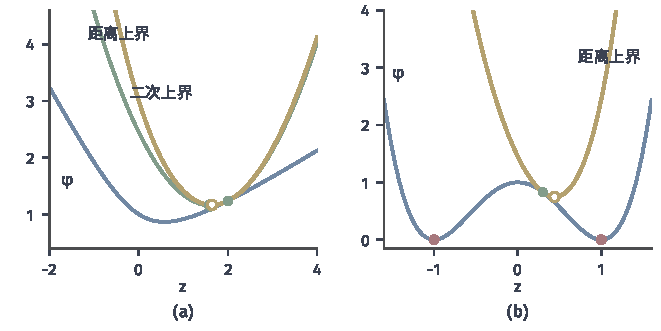
\includegraphics[width=112mm]{figures/05-optimization/04-block-optimization/matplotlib/block-bsum-constructions/figure.pdf}
  \caption{两种块上界的构造。(a)$\varphi(z)=\sqrt{1+z^2}-z/2$（蓝）在$z=2$处的二次上界（绿，$L_J=1$）和保留原函数的距离上界（黄，$\beta=1$），空心点是各自的最小点。(b)非凸函数$\varphi(z)=(z^2-1)^2$有两个最小点（红），在绿点$z=0.3$处加上$\tfrac{10}{2}(z-0.3)^2$后，距离上界（黄）只有一个最小点（空心）。}
  \label{fig:block-bsum-constructions}
\end{BookInlineFigure}

\paragraph{通向块邻近模型}
第三种构造介于两者之间。设目标$F=f+\sum_Jg_J$，光滑项$f$用二次上界代替，可分的非光滑项$g_J$原样保留。这样子问题既保留了$g_J$的结构，又不必处理$f$的复杂形式，这就是第~\ref{sec:block-bpg}节的块邻近模型。

\subsection{与其他块方法的关系}
\label{sec:block-bsum-relations}

把各种更新放进BSUM的框架，能看清谁是谁的特例，也能看清谁不是。图~\ref{fig:block-relations}汇总了这些关系。

\begin{BookInlineFigure}
  \centering
  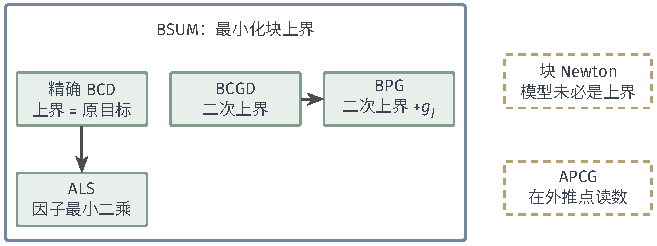
\includegraphics[width=110mm]{figures/05-optimization/04-block-optimization/tikz/block-relations/figure.pdf}
  \caption{BSUM与其他块方法的关系。实线框内是满足块上界条件的更新：精确BCD的上界是条件函数本身，BCGD用二次上界，BPG再保留可分项$g_J$，ALS是因子问题上的精确BCD。黄色虚线框的两种方法一般不满足这些条件，不能未经核验就使用BSUM的下降与收敛保证。}
  \label{fig:block-relations}
\end{BookInlineFigure}

\paragraph{属于BSUM的情形}
当$u_J$就是条件函数时，式~\eqref{eq:block-bsum}就是精确BCD。取式~\eqref{eq:block-ub-quadratic}得到BCGD。下一节的块邻近梯度取光滑部分的二次上界加$g_J$。ALS是因子问题上的精确求解，所以也在框内，但它的关键在于因子结构带来的闭式最小二乘，这一点并不是BSUM框架提供的。

这些关系是按模型的选择和问题的结构形成的交叉，而不是一棵分类树。同一个算法可以从几种角度描述。比如对二次目标，式~\eqref{eq:block-ub-quadratic}取$L_J=Q_{J,J}$（单坐标）时，BCGD和精确BCD就是同一个更新。

\paragraph{不属于BSUM的情形}
一般的块Newton模型不是上界，图~\ref{fig:block-bsum-conditions}(b)已经说明，它需要线搜索或信赖域来保证接受。只有当二阶模型恰好被改造成上界时（比如把Hessian主子矩阵换成一个不小于真实Hessian的矩阵），才回到BSUM。

APCG的模型建立在外推点上，式~\eqref{eq:block-bsum-descent}这样的单调链不成立，手算例子中目标值也确实上升过。它的收敛结论靠的是辅助序列的递推，定理~\ref{thm:block-apcg}不能由BSUM的结论推出。

\section{块邻近梯度（BPG）}
\label{sec:block-bpg}

许多目标是光滑项加上按块可分的非光滑项，例如最小二乘加$\ell_1$正则。接下来要弄清：怎样在一块上同时利用光滑项的梯度和非光滑项的结构，并判断算法何时可以停下来？

设目标是式~\eqref{eq:block-composite}的形式，$g_J$是适当、下半连续的凸函数。第~\ref{chap:nonsmooth-composite-optimization}章已经对完整变量建立了邻近梯度法，这里集中说明分块之后什么地方变了：可分性让邻近映射能逐块计算，步长由块常数决定，残差的含义也不同。第~\ref{sec:block-apcg}小节的APCG是在同样的复合结构上另配了加速递推。

\subsection{块邻近更新}
\label{sec:block-prox-update}

\paragraph{主要思想}
在块$J$上，用二次上界代替光滑项，原样保留非光滑项，得到模型
\begin{equation}
 \begin{aligned}
 u_J(\bm{z};\bm{x})={}&f(\bm{x})+\langle\nabla_Jf(\bm{x}),\bm{z}-\bm{x}_J\rangle+\frac{L_J}{2}\lVert\bm{z}-\bm{x}_J\rVert_2^2\\
 &+g_J(\bm{z})+\sum_{i\neq J}g_i(\bm{x}_i).
 \end{aligned}
 \label{eq:block-prox-model}
\end{equation}

其中只有$\bm{z}$是变量。对前三项配方，最小化$u_J$等价于
\[
 \min_{\bm{z}}\ g_J(\bm{z})+\frac{L_J}{2}\Bigl\lVert\bm{z}-\Bigl(\bm{x}_J-\frac{1}{L_J}\nabla_Jf(\bm{x})\Bigr)\Bigr\rVert_2^2 ,
\]

这正是邻近映射的定义。于是\term{块邻近梯度}（block proximal gradient，BPG）的更新是块梯度步接邻近映射：
\begin{equation}
 \bm{x}_J^{+}=\operatorname{prox}_{g_J/L_J}\Bigl(\bm{x}_J-\frac{1}{L_J}\nabla_Jf(\bm{x})\Bigr).
 \label{eq:block-prox}
\end{equation}
$g_J$是闭凸集$\bm{C}_J$的示性函数时，邻近映射就是到$\bm{C}_J$的投影，式~\eqref{eq:block-prox}成为块投影梯度步，第~\ref{sec:block-coupling}小节的乘积可行域由此纳入同一框架。

\paragraph{完整目标不增}
步长取块常数的倒数，邻近映射精确计算，就有下面的下降量。

\begin{lemma}[块邻近步的下降量]
\label{lem:block-prox-descent}
设$f$可微且满足定义~\ref{def:block-smooth}，$g_J$是适当、下半连续的凸函数，$F(\bm{x})<+\infty$。按式~\eqref{eq:block-prox}更新块$J$，其余块不变，得到$\bm{x}^{+}$。则
\begin{equation}
 F(\bm{x})-F(\bm{x}^{+})\geq\frac{L_J}{2}\lVert\bm{x}_J^{+}-\bm{x}_J\rVert_2^2 .
 \label{eq:block-prox-descent}
\end{equation}
\end{lemma}

\begin{proof}
由式~\eqref{eq:block-quadratic-upper}，$u_J$是块上界，所以$F(\bm{x}^{+})\leq u_J(\bm{x}_J^{+};\bm{x})$。模型的光滑部分带系数$L_J/2$，$g_J$凸，所以$u_J$关于$\bm{z}$是$L_J$强凸的。

$\bm{x}_J^{+}$是$u_J$的最小点，强凸性给出：对任意$\bm{z}$，
\[
 u_J(\bm{z};\bm{x})\geq u_J(\bm{x}_J^{+};\bm{x})+\frac{L_J}{2}\lVert\bm{z}-\bm{x}_J^{+}\rVert_2^2 .
\]

取$\bm{z}=\bm{x}_J$，并由$u_J(\bm{x}_J;\bm{x})=F(\bm{x})$，得到
\[
 F(\bm{x})\geq u_J(\bm{x}_J^{+};\bm{x})+\frac{L_J}{2}\lVert\bm{x}_J-\bm{x}_J^{+}\rVert_2^2\geq F(\bm{x}^{+})+\frac{L_J}{2}\lVert\bm{x}_J-\bm{x}_J^{+}\rVert_2^2 .
\]
\end{proof}

若步长取得比$1/L_J$大，$u_J$就可能不再是上界，下降量不再有保证。这里的“精确”也不是可有可无的条件：邻近子问题解得不准时，要按第~\ref{sec:block-inexact}小节计入误差。

\paragraph{计算过程：套索的单坐标更新}
考虑套索问题，$\gamma>0$，取最小二乘的光滑项和$\ell_1$正则：
\[
 F(\bm{x})=\frac12\lVert\bm{A}\bm{x}-\bm{b}\rVert_2^2+\gamma\lVert\bm{x}\rVert_1 .
\]
取坐标为块，$g_j=\gamma\lvert\cdot\rvert$可分，$\gamma\lvert\cdot\rvert/L_j$的邻近映射是软阈值
\begin{equation}
 S_{\tau}(v)=\operatorname{sign}(v)\max\{\lvert v\rvert-\tau,\,0\},\qquad \tau=\frac{\gamma}{L_j}.
 \label{eq:block-soft-threshold}
\end{equation}
于是式~\eqref{eq:block-prox}成为
\begin{equation}
 x_j^{+}=S_{\gamma/L_j}\Bigl(x_j-\frac{1}{L_j}\bm{a}_j^\top\bm{r}\Bigr),\qquad L_j=\lVert\bm{a}_j\rVert_2^2 .
 \label{eq:block-lasso-update}
\end{equation}
这时光滑项的条件函数是抛物线，上界等于它，式~\eqref{eq:block-lasso-update}也是精确块解。

\needspace{6\baselineskip}
\paragraph{变量}
\begin{itemize}
 \item $\bm{x}$：当前系数；$\bm{r}=\bm{A}\bm{x}-\bm{b}$：残差，每次更新后维护。
 \item $L_j$：各列的平方范数，事先算好；$\gamma$：正则系数。
\end{itemize}

\paragraph{初始化}
下面用与前面相同的$\bm{A}$，并取以下数据进行演示：
\[
 \bm{b}=(4,2,-1),\qquad \gamma=1,\qquad \bm{x}^{(0)}=(3,4).
\]
于是$L_1=L_2=2$，阈值$\tau=\tfrac12$，初始残差$\bm{r}=(3,1,5)$，目标值$F=24.5$。

\paragraph{每轮更新}
循环取坐标$j=1,2$，每次按式~\eqref{eq:block-lasso-update}更新$x_j$，再更新残差$\bm{r}\leftarrow\bm{r}+(x_j^{+}-x_j)\bm{a}_j$。

\begin{enumerate}
 \item 第一轮，$j=1$：$\bm{a}_1^\top\bm{r}=4$，软阈值的输入是$3-2=1$，于是
 \[
  x_1=0.5,\qquad \bm{r}=(0.5,-1.5,5),\qquad F=18.25 .
 \]
 \item 第一轮，$j=2$：$\bm{a}_2^\top\bm{r}=5.5$，输入是$4-2.75=1.25$，于是
 \[
  x_2=0.75,\qquad \bm{r}=(-2.75,-1.5,1.75),\qquad F=7.6875 .
 \]
 \item 第二轮，$j=1$：$\bm{a}_1^\top\bm{r}=-4.25$，输入是$0.5+2.125=2.625$，于是
 \[
  x_1=2.125,\qquad \bm{r}=(-1.125,0.125,1.75),\qquad F=5.046875 .
 \]
 \item 第二轮，$j=2$：$\bm{a}_2^\top\bm{r}=0.625$，输入是$0.75-0.3125=0.4375$，小于阈值，于是
 \[
  x_2=0,\qquad \bm{r}=(-1.875,0.125,1),\qquad F=4.390625 .
 \]
 \item 第三轮，$j=1$：$\bm{a}_1^\top\bm{r}=-1.75$，输入是$2.125+0.875=3$，于是
 \[
  x_1=2.5,\qquad \bm{r}=(-1.5,0.5,1),\qquad F=4.25 .
 \]
 \item 第三轮，$j=2$：$\bm{a}_2^\top\bm{r}=-0.5$，输入是$0+0.25=0.25$，仍小于阈值，$x_2$保持为$0$。
\end{enumerate}

此时两个坐标都不再变化，迭代结束，最终得到$\bm{x}=(2.5,0)$，$F=4.25$。图~\ref{fig:block-soft-threshold}(a)是软阈值函数，(b)是这条路径。第二轮之后$x_2$被压到$0$并留在那里，这就是$\ell_1$正则产生稀疏解的方式。

\begin{BookInlineFigure}
  \centering
  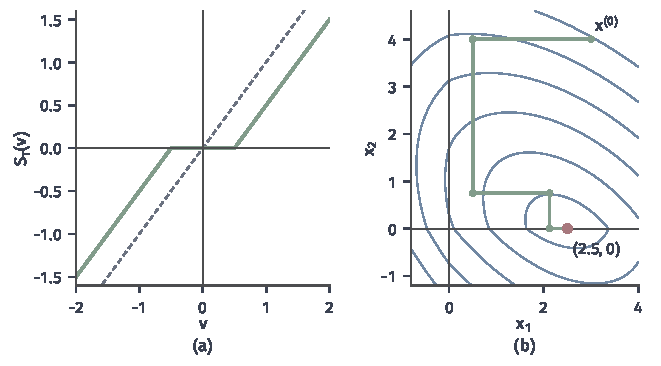
\includegraphics[width=112mm]{figures/05-optimization/04-block-optimization/matplotlib/block-soft-threshold/figure.pdf}
  \caption{套索的坐标更新。(a)软阈值函数$S_{1/2}(v)$（绿），灰色虚线是恒等映射，$\lvert v\rvert\leq\tfrac12$的输入被压成$0$。(b)文中的例子：蓝色是复合目标的等高线，绿色折线是循环更新的路径，第二轮把$x_2$压到坐标轴上，红点是解$(2.5,0)$。}
  \label{fig:block-soft-threshold}
\end{BookInlineFigure}

\paragraph{可分性的边界}
上面每一步能单独计算，靠的是非光滑项能拆成$\sum_jg_j(x_j)$。对式~\eqref{eq:block-nonsmooth-example}这样的不可分项，把一块的条件函数写出来仍是可以的，比如固定$v$后对$u$的邻近子问题，但它的结果依赖其他块，算法也就可能如第~\ref{sec:block-coupling}小节那样停滞。逐块计算的前提和逐块最优性能合成整体驻点的前提，是同一个可分性。

\subsection{块邻近残差}
\label{sec:block-prox-residual}

\paragraph{要回答的问题}
光滑时用偏梯度判断一块是否调好了。有非光滑项时偏梯度不再归零，比如解$(2.5,0)$处第二个坐标的偏导数是$-0.5$，不是$0$，该坐标却已经最优。需要一个既能处理非光滑项又能计算的量。

\begin{definition}[块梯度映射]
\label{def:block-gradient-mapping}
设$\alpha>0$，定义块$J$的\term{块梯度映射}（block gradient mapping）为
\begin{equation}
 \bm{G}_J(\bm{x})=\frac{1}{\alpha}\Bigl(\bm{x}_J-\operatorname{prox}_{\alpha g_J}\bigl(\bm{x}_J-\alpha\nabla_Jf(\bm{x})\bigr)\Bigr).
 \label{eq:block-gradient-mapping}
\end{equation}
\end{definition}

它是块邻近步的位移除以步长。$g_J\equiv0$时就是偏梯度$\nabla_Jf(\bm{x})$，所以它是偏梯度的自然推广。

\paragraph{全部为零即复合驻点}
由邻近映射的最优性条件可以读出这个量的含义。记$\bm{p}=\operatorname{prox}_{\alpha g_J}(\bm{v})$，则$\bm{p}$满足$(\bm{v}-\bm{p})/\alpha\in\partial g_J(\bm{p})$，其中$\partial g_J$是次微分。取$\bm{v}=\bm{x}_J-\alpha\nabla_Jf(\bm{x})$，$\bm{G}_J(\bm{x})=\bm{0}$就是$\bm{p}=\bm{x}_J$，代入得到
\[
 -\nabla_Jf(\bm{x})\in\partial g_J(\bm{x}_J).
\]

反过来，若上式成立，$\bm{x}_J$满足邻近子问题的最优性条件，邻近映射的解唯一，所以$\bm{p}=\bm{x}_J$。

因此全部块的映射同时为零，等价于每块都有$-\nabla_Jf(\bm{x})\in\partial g_J(\bm{x}_J)$。由$g$按块可分，次微分是各块次微分的乘积，上面$B$个包含关系合起来就是
\begin{equation}
 \bm{0}\in\nabla f(\bm{x})+\partial g(\bm{x}).
 \label{eq:block-composite-stationary}
\end{equation}
这是复合目标的驻点条件。$f$凸时，由引理~\ref{lem:block-joint-convex}的论证，它也是全局最优条件。

\paragraph{刚更新块的残差}
实际运行中还有一个容易出错的地方：不要拿刚更新块的残差代替完整残差。例中取$\alpha=\tfrac12$，看前两步的残差，其中$\bm{G}_J$的值都按更新后的点重新计算：
\[
 \begin{aligned}
 \bm{x}=(3,4):&\quad G_1=5,\quad G_2=8,\\
 \bm{x}=(0.5,4):&\quad G_1=0,\quad G_2=6.5,\\
 \bm{x}=(0.5,0.75):&\quad G_1=-3.25,\quad G_2=0.
 \end{aligned}
\]
第二行刚更新了$x_1$，$G_1$变成$0$。但第三行更新$x_2$之后，$G_1$又变成了$-3.25$：$x_1$在新的$x_2$下不再是最优的。

一块的残差只反映这一块在当时的状况，其他块一变，先前算出的残差就过期了。完整驻点残差要求所有块在同一点上重新计算，停止准则应当用它，或者至少在一轮结束后重算一次。

图~\ref{fig:block-residual-stale}对比了两个量。黄点是每次更新前对被更新块算出的残差，绿线是当时所有块的完整残差。黄点常常比绿线小一到两个数量级，个别的还接近零，这时只看单块残差就会过早停止。

\begin{BookInlineFigure}
  \centering
  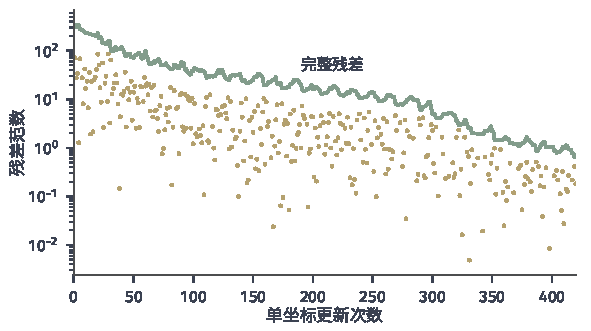
\includegraphics[width=100mm]{figures/05-optimization/04-block-optimization/matplotlib/block-residual-stale/figure.pdf}
  \caption{单块残差与完整残差。$N=60$、$n=30$的套索问题（列之间相关，$\gamma=2$），循环单坐标更新$14$轮。绿线是全部块的残差范数，黄点是每次被更新那一块在更新前的残差绝对值（$\alpha=1/L_j$）。残差为零的点因对数坐标未画出。}
  \label{fig:block-residual-stale}
\end{BookInlineFigure}

\section{实现与收敛}
\label{sec:block-implementation}

前面几节给出了更新公式。本节把它们放回实际运行的环境，回答：更新怎样读值，内层要解到多准，算法能保证什么，总计算量是否真的省了？下面的结论都与具体的选块规则、模型条件和误差要求绑定，评价进展时统一看完整目标。

\subsection{串行与并行}
\label{sec:block-parallel}

\paragraph{串行读新值，并行读旧值}
串行时，每一块读取的都是已经更新过的最新值。并行时，多块基于同一个旧点同时计算，然后同时写入。这看起来只差一点，实际上改变了算法的性质：串行步长的保证建立在“只有一块变化”上，而并行时变化的是几块的和。

用最小的例子看。目标是
\[
 f(u,v)=\frac12(u+v)^2,\qquad (u,v)=(1,1).
\]
每个坐标的块光滑常数都是$1$。串行时，先更新$u$，得$u=1-2=-1$，到达$(-1,1)$，目标值$0$，已经最优。

并行时，两个坐标都读$u+v=2$，都走同样的一步，得到
\[
 (u,v)=(1,1)-(2,2)=(-1,-1),
\]
目标值仍是$2$。下一步又回到$(1,1)$，迭代在这两点之间振荡，永远不动。每一块单独都沿下降方向走，合起来却越过了最低点。图~\ref{fig:block-parallel-jacobi}(a)是这条路径。

\paragraph{覆盖同时变化的联合上界}
上界~\eqref{eq:block-quadratic-upper}只对一块变化成立。要保证并行步，需要一个覆盖几块同时变化的上界。下面的引理说明，对凸目标，只需把步长缩小到同时更新块数的倒数。

\begin{lemma}[并行更新的联合上界]
\label{lem:block-parallel-upper}
设$f$是凸函数，且满足定义~\ref{def:block-smooth}。$\mathcal{S}$是含$\tau$个块的集合，$\bm{h}_J\in\mathbb{R}^{\lvert J\rvert}$（$J\in\mathcal{S}$）。则
\begin{equation}
 f\Bigl(\bm{x}+\sum_{J\in\mathcal{S}}\bm{U}_J\bm{h}_J\Bigr)
 \leq f(\bm{x})+\sum_{J\in\mathcal{S}}\langle\nabla_Jf(\bm{x}),\bm{h}_J\rangle+\frac{\tau}{2}\sum_{J\in\mathcal{S}}L_J\lVert\bm{h}_J\rVert_2^2 .
 \label{eq:block-parallel-upper}
\end{equation}
\end{lemma}

\begin{proof}
把位移写成$\tau$个块方向的平均：
\[
 \bm{x}+\sum_{J\in\mathcal{S}}\bm{U}_J\bm{h}_J=\frac{1}{\tau}\sum_{J\in\mathcal{S}}\bigl(\bm{x}+\tau\bm{U}_J\bm{h}_J\bigr).
\]

由$f$的凸性，
\[
 f\Bigl(\bm{x}+\sum_{J\in\mathcal{S}}\bm{U}_J\bm{h}_J\Bigr)\leq\frac{1}{\tau}\sum_{J\in\mathcal{S}}f\bigl(\bm{x}+\tau\bm{U}_J\bm{h}_J\bigr).
\]

对每一项用上界~\eqref{eq:block-quadratic-upper}，位移取$\tau\bm{h}_J$：
\[
 f\bigl(\bm{x}+\tau\bm{U}_J\bm{h}_J\bigr)\leq f(\bm{x})+\tau\langle\nabla_Jf(\bm{x}),\bm{h}_J\rangle+\frac{L_J\tau^2}{2}\lVert\bm{h}_J\rVert_2^2 .
\]
代入后除以$\tau$，即得式~\eqref{eq:block-parallel-upper}。
\end{proof}

式~\eqref{eq:block-parallel-upper}的右边对各块可分，分别最小化，得到每块的并行步长$1/(\tau L_J)$，并且保证下降量至少是
\begin{equation}
 \frac{1}{2\tau}\sum_{J\in\mathcal{S}}\frac{\lVert\nabla_Jf(\bm{x})\rVert_2^2}{L_J} .
 \label{eq:block-parallel-decrease}
\end{equation}
例中$\tau=2$，步长是$\tfrac12$，两个坐标都走$-1$，一步到$(0,0)$。

这个因子$\tau$偏保守。对最小二乘，若$\bm{A}$的每一行最多有$\omega$个非零元，由Cauchy--Schwarz不等式，第$i$行满足
\[
 \Bigl(\sum_ja_{i,j}h_j\Bigr)^2\leq\omega\sum_ja_{i,j}^2h_j^2 .
\]
对所有行求和，二次项不超过$\omega\sum_jL_jh_j^2$，所以因子可以取$\min\{\tau,\omega\}$。变量之间的耦合越稀疏，并行越接近串行的效率。例中$\bm{A}$的第一行有两个非零元，$\omega=2$。

图~\ref{fig:block-parallel-jacobi}(b)是三变量的例子，$\bm{Q}=0.25\,\bm{I}+0.75\,\bm{1}\bm{1}^\top$。串行步长$\alpha=1$（$L_j=1$）用于并行时目标值发散，缩小到$\alpha=\tfrac13$后单调下降，但慢于串行。

\begin{BookInlineFigure}
  \centering
  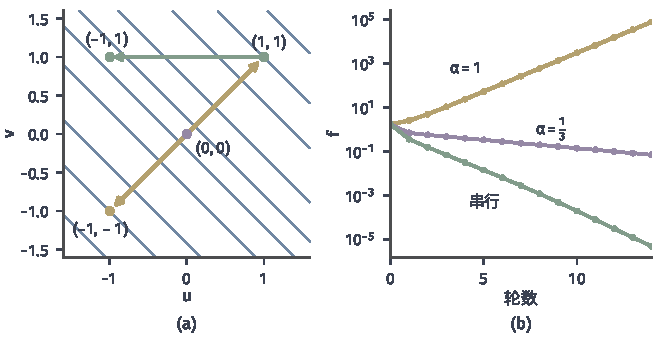
\includegraphics[width=112mm]{figures/05-optimization/04-block-optimization/matplotlib/block-parallel-jacobi/figure.pdf}
  \caption{串行与并行。(a)$f=\tfrac12(u+v)^2$从$(1,1)$出发：绿色是串行一步到达$(-1,1)$；黄色是并行且步长$1$，在$(1,1)$与$(-1,-1)$间振荡；紫点是并行且步长$\tfrac12$的结果$(0,0)$。(b)$n=3$、$\bm{Q}=0.25\,\bm{I}+0.75\,\bm{1}\bm{1}^\top$时目标值随轮数的变化：黄线是并行且步长$1$，紫线是并行且步长$\tfrac13$，绿线是串行且步长$1$。}
  \label{fig:block-parallel-jacobi}
\end{BookInlineFigure}

\paragraph{实现条件}
同步并行要在每轮末等所有块写完，这一等待有实际的时间成本。共享残差时，多个块同时写$\bm{r}$要处理写冲突；块的数据不重叠时才能完全并行。若不做同步，块会读到别的块更新到一半的旧值，这时上面的引理不再适用，需要另外分析读取延迟。

\subsection{子问题的求解精度}
\label{sec:block-inexact}

\paragraph{把误差计入下降量}
块子问题常常只能迭代求解。设$m$是当前块的模型（精确BCD时就是条件函数），$\bm{z}^\star$是模型的最小点。近似解$\tilde{\bm{z}}$的模型值误差为
\begin{equation}
 m(\tilde{\bm{z}})\leq m(\bm{z}^\star)+\varepsilon .
 \label{eq:block-inexact}
\end{equation}
若$m$是块上界，由上界与相等条件，近似解带来的完整目标下降至少是
\begin{equation}
 F(\bm{x})-F(\bm{x}^{+})\geq\bigl(m(\bm{x}_J)-m(\bm{z}^\star)\bigr)-\varepsilon .
 \label{eq:block-inexact-descent}
\end{equation}
也就是精确解的模型下降量，减去误差。

\paragraph{两种接受条件}
区分两种条件。“不劣于当前点”即$m(\tilde{\bm{z}})\leq m(\bm{x}_J)$，它能维持单调性，但太弱：$\tilde{\bm{z}}=\bm{x}_J$也能通过，一点进展都没有。

支持长期进展的是相对精度：取$0\leq\eta<1$，要求
\begin{equation}
 m(\tilde{\bm{z}})-m(\bm{z}^\star)\leq\eta\bigl(m(\bm{x}_J)-m(\bm{z}^\star)\bigr).
 \label{eq:block-relative-accuracy}
\end{equation}
由式~\eqref{eq:block-inexact-descent}，这样的近似解保留精确解模型下降量的$(1-\eta)$倍。精确解的所有保底下降界乘以$(1-\eta)$仍然成立，收敛速率只差一个常数因子。

\paragraph{怎样测量误差}
$m(\bm{z}^\star)$通常不知道，需要可计算的上界。设子问题是正定二次函数，$\bm{P}$是对称正定矩阵，且$\bm{P}\succeq\sigma\bm{I}$，$\sigma>0$：
\[
 m(\bm{z})=\frac12\bm{z}^\top\bm{P}\bm{z}-\bm{q}^\top\bm{z}.
\]
梯度残差$\bm{s}=\bm{P}\tilde{\bm{z}}-\bm{q}$是可以计算的。由$\bm{z}^\star=\bm{P}^{-1}\bm{q}$，得$\tilde{\bm{z}}-\bm{z}^\star=\bm{P}^{-1}\bm{s}$。二次函数在最小点附近精确地展开为
\[
 m(\tilde{\bm{z}})-m(\bm{z}^\star)=\frac12(\tilde{\bm{z}}-\bm{z}^\star)^\top\bm{P}(\tilde{\bm{z}}-\bm{z}^\star)=\frac12\bm{s}^\top\bm{P}^{-1}\bm{s}.
\]

再由$\bm{P}^{-1}$的最大特征值不超过$1/\sigma$，得到
\begin{equation}
 m(\tilde{\bm{z}})-m(\bm{z}^\star)\leq\frac{\lVert\bm{s}\rVert_2^2}{2\sigma}.
 \label{eq:block-residual-bound}
\end{equation}
例中$x_2=4$时，条件函数是$z^2+4z+16$，所以$P=2$，$q=-4$，$\sigma=2$。取$\tilde{z}=-1.9$，残差$s=2(-1.9)+4=0.2$，误差确实是$(-1.9+2)^2=0.01$，而界$s^2/(2\sigma)=0.04/4=0.01$恰好取到。

\paragraph{固定绝对误差的精度限制}
若每步都有相同的绝对误差$\varepsilon$，长期结果就有下限。设无误差时有收缩$E^{(t+1)}\leq(1-\rho)E^{(t)}$，$0<\rho<1$，这里$E^{(t)}$是目标差或其期望。由式~\eqref{eq:block-inexact-descent}，有误差时变成
\[
 E^{(t+1)}\leq(1-\rho)E^{(t)}+\varepsilon .
\]
展开这个递推，并对等比级数求和，得到
\begin{equation}
 E^{(T)}\leq(1-\rho)^TE^{(0)}+\frac{\varepsilon}{\rho}.
 \label{eq:block-error-floor}
\end{equation}
第一项趋于零，第二项不会消失，算法最终停在一个与$\varepsilon/\rho$同量级的平台上。图~\ref{fig:block-inexact-accuracy}的黄线就是这个平台，紫线用相对精度~\eqref{eq:block-relative-accuracy}的同类要求，一直下降，只是比精确解慢一些。

\begin{BookInlineFigure}
  \centering
  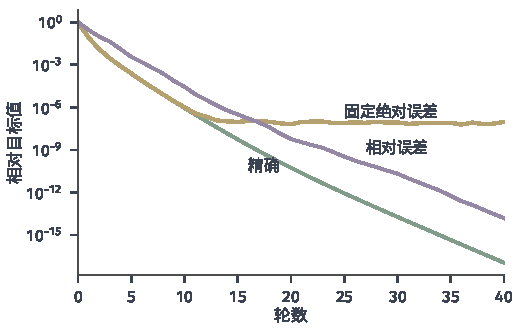
\includegraphics[width=88mm]{figures/05-optimization/04-block-optimization/matplotlib/block-inexact-accuracy/figure.pdf}
  \caption{块子问题误差的影响。$n=40$的正定二次目标，每块$8$个变量，循环更新。绿线是精确块解；黄线的每次块解有固定的残差范数$10^{-3}$，目标值停在平台上；紫线的残差范数取当前偏梯度范数的一半，仍线性收敛。}
  \label{fig:block-inexact-accuracy}
\end{BookInlineFigure}

\paragraph{内层成本与解的复用}
相对精度也有成本。把一块解到较高精度需要更多内层迭代，而上一轮的块解是内层求解的好起点，这称为热启动；固定曲率时，矩阵分解还能重复使用。接受标准定得太严，一步就要做很多无用的内层迭代；定得太松，外层要多走好多轮。两者的总和才是要比较的量。

\subsection{收敛保证}
\label{sec:block-convergence}

\paragraph{三个不同的问题}
“算法收敛”可以指三件不同的事，由弱到强依次是：目标值序列收敛；迭代点的聚点是驻点；整个迭代点序列收敛到一点。下面分别看各需要什么条件。

\paragraph{目标值收敛}
只要每步不增且目标有下界，目标值序列就收敛。精确块更新由引理~\ref{lem:block-exact-descent}满足单调性，BCGD由式~\eqref{eq:block-bcgd-decrease}满足，BSUM由式~\eqref{eq:block-bsum-descent}满足，BPG由式~\eqref{eq:block-prox-descent}满足。这个结论很弱，它不说明目标值收敛到哪里，更不说明点收敛。

\paragraph{聚点驻定}
聚点的性质需要逐条检查四件事：块访问，即每一块都被反复更新；解的选择，即子问题的解有确定的规则，这里要求唯一；水平集条件，使迭代有聚点；以及分块的最优性条件能否合成整体驻点条件。

下面给出循环规则下的结论。设$\bm{C}$是闭凸集的乘积，$F$在$\bm{C}$上连续。

\begin{theorem}[循环BSUM的聚点]
\label{thm:block-bsum-limit}
设$\bm{x}^{(0)}\in\bm{C}$，下水平集
\begin{equation}
 \bm{S}=\{\bm{x}\in\bm{C}:F(\bm{x})\leq F(\bm{x}^{(0)})\}
 \label{eq:block-level-set}
\end{equation}
是紧集。设每个块的$u_J$满足定义~\ref{def:block-upper-bound}，且对每个$\bm{y}\in\bm{S}$，$u_J(\cdot;\bm{y})$在$\bm{C}_J$上有唯一的最小点。按固定顺序循环更新各块，则每轮开始时的点列$\{\bm{x}^{(t)}\}$有聚点，并且每个聚点$\bar{\bm{x}}$满足
\begin{equation}
 \bar{\bm{x}}_J=\argmin_{\bm{z}\in\bm{C}_J}u_J(\bm{z};\bar{\bm{x}})\quad\text{对每个块}\ J,
 \label{eq:block-limit-fixed}
\end{equation}
\begin{equation}
 F'(\bar{\bm{x}};\bm{U}_J\bm{d})\geq0\quad\text{对每个块}\ J\ \text{和满足}\ \bar{\bm{x}}_J+\bm{d}\in\bm{C}_J\ \text{的}\ \bm{d}.
 \label{eq:block-limit-directional}
\end{equation}
\end{theorem}

\begin{proof}
记$M_J(\bm{y})$为只把$\bm{y}$的块$J$替换成$u_J(\cdot;\bm{y})$的最小点得到的点。由下降链~\eqref{eq:block-bsum-descent}，$M_J$把$\bm{S}$映入$\bm{S}$，迭代始终留在$\bm{S}$中。$\bm{S}$紧，所以聚点存在，$F(\bm{x}^{(t)})$单调有界而收敛到某个$\bar{F}$，由连续性，每个聚点满足$F(\bar{\bm{x}})=\bar{F}$。

先证$M_J$在$\bm{S}$上连续。设$\bm{y}^{(k)}\to\bm{y}$，$\bm{y}^{(k)}\in\bm{S}$，任取$M_J(\bm{y}^{(k)})$的一个收敛子列，极限$\bar{\bm{z}}$在$\bm{S}$中，且只在块$J$上与$\bm{y}$不同。对任意$\bm{w}\in\bm{C}_J$，有
\[
 u_J\bigl(M_J(\bm{y}^{(k)})_J;\bm{y}^{(k)}\bigr)\leq u_J(\bm{w};\bm{y}^{(k)}).
\]
令$k\to\infty$，由$u_J$的连续性，$\bar{\bm{z}}_J$是$u_J(\cdot;\bm{y})$的最小点，由唯一性，$\bar{\bm{z}}=M_J(\bm{y})$。紧集中的序列每个收敛子列的极限都相同，所以$M_J(\bm{y}^{(k)})\to M_J(\bm{y})$。

再设子列$\bm{x}^{(t_j)}\to\bar{\bm{x}}$，块的顺序是$J_1,\ldots,J_B$。令$\bm{z}^{j,0}=\bm{x}^{(t_j)}$，$\bm{z}^{j,k}=M_{J_k}(\bm{z}^{j,k-1})$。下面对$k$归纳证明$\bm{z}^{j,k}\to\bar{\bm{x}}$（$j\to\infty$）。设$\bm{z}^{j,k-1}\to\bar{\bm{x}}$，由$M_{J_k}$的连续性，$\bm{z}^{j,k}$收敛到点
\[
 \bar{\bm{w}}=M_{J_k}(\bar{\bm{x}}).
\]

由单调性，
\[
 F(\bm{x}^{(t_j+1)})\leq F(\bm{z}^{j,k})\leq F(\bm{x}^{(t_j)}),
\]
两端都趋于$\bar{F}$，所以$F(\bar{\bm{w}})=\bar{F}$。再由下降链，
\[
 \bar{F}=F(\bar{\bm{w}})\leq u_{J_k}(\bar{\bm{w}}_{J_k};\bar{\bm{x}})\leq u_{J_k}(\bar{\bm{x}}_{J_k};\bar{\bm{x}})=F(\bar{\bm{x}})=\bar{F}.
\]
这表明$\bar{\bm{x}}_{J_k}$也是$u_{J_k}(\cdot;\bar{\bm{x}})$的最小点。由唯一性，$\bar{\bm{w}}=\bar{\bm{x}}$，归纳完成，并且式~\eqref{eq:block-limit-fixed}对每个$J_k$成立。

最后，$\bar{\bm{x}}_J$最小化$u_J(\cdot;\bar{\bm{x}})$，$\bm{C}_J$是凸集，所以沿任何可行方向的方向导数非负。由一阶条件~\eqref{eq:block-ub-derivative}，这就是式~\eqref{eq:block-limit-directional}。
\end{proof}

取$u_J$为条件函数，定理就覆盖了精确BCD。定理中的条件各有用处：紧性让聚点存在；唯一性决定了不动点论证中的$\bar{\bm{w}}=\bar{\bm{x}}$；循环访问保证每个块都被访问到。“每隔固定步数每块至少访问一次”的规则也能用同样的论证。

\paragraph{唯一性去掉会怎样}
最小点不唯一时，聚点可以不是驻点。一个经典的三变量例子是
\[
 f(\bm{x})=-(x_1x_2+x_2x_3+x_3x_1)+\sum_{i=1}^{3}(\lvert x_i\rvert-1)_+^2 ,
\]
其中$(s)_+=\max\{s,0\}$。固定其余两个变量，令和为$s\neq0$时，$x_1$的最小点唯一，是$\operatorname{sign}(s)(1+\lvert s\rvert/2)$；$s=0$时，$[-1,1]$上每一点都是最小点。

从下面的起点出发循环更新，$\epsilon>0$：
\[
 \bm{x}^{(0)}=\Bigl(-1-\epsilon,\ 1+\frac{\epsilon}{2},\ -1-\frac{\epsilon}{4}\Bigr).
\]
三步之后的三个坐标依次是
\[
 x_1=1+\frac{\epsilon}{8},\qquad x_2=-1-\frac{\epsilon}{16},\qquad x_3=1+\frac{\epsilon}{32}.
\]
每次偏离$\pm1$的量缩小到一半，符号不断翻转，迭代点沿立方体的六个顶点循环，聚点是这些顶点。

顶点不是驻点，比如$(1,1,-1)$处$\partial_3f=-2$，$\partial_1f=\partial_2f=0$。问题正出在极限处$s=0$：条件子问题的最小点不再唯一，$M_J$不再连续，定理的论证在这里断开。这个例子的目标也没有下界，这里关心的是解的选择造成的现象，水平集条件并不是它失效的主因。

\paragraph{合成整体驻点}
式~\eqref{eq:block-limit-directional}只说沿块方向的方向导数非负。能否合成整体驻点，要看方向导数在块间是否可加。$F$可微时，方向导数按块相加：
\[
 F'(\bar{\bm{x}};\bm{d})=\sum_J\langle\nabla_JF(\bar{\bm{x}}),\bm{d}_J\rangle ,
\]
每一项非负，和也非负，这就是闭凸可行域上的驻点条件。

$F=f+\sum_Jg_J$且$g_J$凸时，方向导数同样按块相加，结论也成立；$F$凸时由此得到全局最优。例~\eqref{eq:block-nonsmooth-example}的方向导数不能按块分开，这一步失败。

\paragraph{整列收敛}
聚点驻定仍然允许序列在几个驻点之间徘徊。整列收敛到一点需要更强的条件，典型的是强凸性。若$F$是$\mu$强凸的且$F(\bm{x}^{(t)})\to F^\star$，则由
\[
 \frac{\mu}{2}\lVert\bm{x}^{(t)}-\bm{x}^\star\rVert_2^2\leq F(\bm{x}^{(t)})-F^\star
\]
得到$\bm{x}^{(t)}\to\bm{x}^\star$。非强凸时需要借助目标在解附近的增长性质，这超出本章范围。

\paragraph{随机BCGD的有限步界}
上面的结论都是渐近的，下面给出有限步的结果。这里考虑独立均匀选块、使用精确偏梯度的BCGD，分析的关键仍是单步的平均下降。

\begin{theorem}[随机BCGD的收敛率]
\label{thm:block-rbcgd}
设$f:\mathbb{R}^n\to\mathbb{R}$有下界$f^\star$，关于每一块是$L_J$光滑的，记$L_{\max}=\max_JL_J$。每步与历史独立地均匀抽取一块，按式~\eqref{eq:block-bcgd}更新。则有
\begin{equation}
 \mathbb{E}\bigl[f(\bm{x}^{(t+1)})\mid\bm{x}^{(t)}\bigr]\leq f(\bm{x}^{(t)})-\frac{1}{2BL_{\max}}\lVert\nabla f(\bm{x}^{(t)})\rVert_2^2 ,
 \label{eq:block-rbcgd-one-step}
\end{equation}
\begin{equation}
 \min_{0\leq t<T}\mathbb{E}\lVert\nabla f(\bm{x}^{(t)})\rVert_2^2\leq\frac{2BL_{\max}\bigl(f(\bm{x}^{(0)})-f^\star\bigr)}{T}.
 \label{eq:block-rbcgd-gradient}
\end{equation}
若$f$还是$\mu$强凸的，则
\begin{equation}
 \mathbb{E}f(\bm{x}^{(T)})-f^\star\leq\Bigl(1-\frac{\mu}{BL_{\max}}\Bigr)^{T}\bigl(f(\bm{x}^{(0)})-f^\star\bigr).
 \label{eq:block-rbcgd-linear}
\end{equation}
\end{theorem}

\begin{proof}
抽到块$J$的概率是$1/B$，由式~\eqref{eq:block-bcgd-decrease}，此时下降量至少是$\lVert\nabla_Jf\rVert_2^2/(2L_J)$。对$B$个块取平均，并用$L_J\leq L_{\max}$，得到
\[
 \mathbb{E}\bigl[f(\bm{x}^{(t+1)})\mid\bm{x}^{(t)}\bigr]\leq f(\bm{x}^{(t)})-\frac{1}{2BL_{\max}}\sum_J\lVert\nabla_Jf(\bm{x}^{(t)})\rVert_2^2 .
\]
各块的下标互不重叠且并起来是全部下标，所以
\[
 \sum_J\lVert\nabla_Jf\rVert_2^2=\lVert\nabla f\rVert_2^2 ,
\]
这就是式~\eqref{eq:block-rbcgd-one-step}。

对式~\eqref{eq:block-rbcgd-one-step}取全期望，并对$t=0,\ldots,T-1$求和，左右两边的目标值相消，得到
\[
 \frac{1}{2BL_{\max}}\sum_{t=0}^{T-1}\mathbb{E}\lVert\nabla f(\bm{x}^{(t)})\rVert_2^2\leq f(\bm{x}^{(0)})-\mathbb{E}f(\bm{x}^{(T)})\leq f(\bm{x}^{(0)})-f^\star .
\]
最小值不超过平均值，移项即得式~\eqref{eq:block-rbcgd-gradient}。

强凸时，把强凸下界对$\bm{y}$取最小：
\[
 \begin{aligned}
 f^\star&\geq\min_{\bm{y}}\Bigl\{f(\bm{x})+\langle\nabla f(\bm{x}),\bm{y}-\bm{x}\rangle+\frac{\mu}{2}\lVert\bm{y}-\bm{x}\rVert_2^2\Bigr\}\\
 &=f(\bm{x})-\frac{1}{2\mu}\lVert\nabla f(\bm{x})\rVert_2^2 ,
 \end{aligned}
\]
也就是
\[
 \lVert\nabla f(\bm{x})\rVert_2^2\geq2\mu\bigl(f(\bm{x})-f^\star\bigr).
\]
把它代入式~\eqref{eq:block-rbcgd-one-step}，两边减去$f^\star$，得到
\[
 \mathbb{E}\bigl[f(\bm{x}^{(t+1)})-f^\star\mid\bm{x}^{(t)}\bigr]\leq\Bigl(1-\frac{\mu}{BL_{\max}}\Bigr)\bigl(f(\bm{x}^{(t)})-f^\star\bigr).
\]
取全期望并反复使用即得式~\eqref{eq:block-rbcgd-linear}。
\end{proof}

例中$B=2$，$L_{\max}=2$，$\mu=1$，因子是$\tfrac34$。从$f=37$出发一步后，定理的上界是$27.75$，实际的平均值是$9.375$：定理只用了最坏的块光滑常数，实际情况好得多。

$B$次更新的成本约等于一次全梯度，这时因子约为$1-\mu/L_{\max}$。与第~\ref{chap:first-order-methods}章梯度下降每步的$1-\mu/L$相比，$L_{\max}$越小于$L$，块方法越有优势\scite{nesterov2012efficiency}。式~\eqref{eq:block-constant-order}中的$L_j\leq L$保证了这个比较不会反过来。

\paragraph{加速方法另当别论}
定理~\ref{thm:block-rbcgd}的论证依赖于每步的单调下降。APCG的$F(\bm{x}^{(t)})$不是单调的，这里的论证用不上，定理~\ref{thm:block-apcg}的结论要靠辅助序列的递推才能得到。

\subsection{计算成本}
\label{sec:block-cost}

\paragraph{一次更新的读取量}
最后回到开头的问题：计算真的省了吗？以稠密的$\bm{A}\in\mathbb{R}^{N\times n}$为例，比较三种操作的运算量（只数乘法）。一次单坐标更新要读$\bm{a}_j^\top\bm{r}$和更新$\bm{r}$，各需$N$次；一次完整遍历$n$个坐标，一次全梯度要算$\bm{A}\bm{x}$和$\bm{A}^\top\bm{r}$，结果如下表。

\begin{BookInlineTable}
\centering
\begin{tabular}{lll}
\toprule
操作 & 稠密$\bm{A}$ & 稀疏$\bm{A}$\\
\midrule
一次单坐标更新 & $2N$ & $2\operatorname{nnz}(\bm{a}_j)$\\
一轮（$n$次更新） & $2Nn$ & $2\operatorname{nnz}(\bm{A})$\\
一次全梯度 & $2Nn$ & $2\operatorname{nnz}(\bm{A})$\\
\bottomrule
\end{tabular}
\end{BookInlineTable}

由此可知，维护残差之后，一轮坐标更新和一次全梯度的成本相同。若没有维护残差，每次更新都重算$\bm{A}\bm{x}$，一轮的成本就变成全梯度的$n$倍，优势全失。

例中$\bm{A}$每列两个非零元，一次更新要$4$次乘法，一轮$8$次，一次全梯度也是$8$次。花同样的计算，一轮循环坐标下降把目标值乘以$\tfrac{1}{16}$，最优固定步长的梯度下降每步只乘以$\tfrac14$（$\kappa=3$，由第~\ref{chap:first-order-methods}章的结论，$((\kappa-1)/(\kappa+1))^2=\tfrac14$）。

\paragraph{完整的成本清单}
比较几种方法要用同一个目标和同一个精度要求，并把下表中的所有项计入，只算迭代次数或只算单步代价都会得出错误的结论。

\begin{BookInlineTable}
\centering
\begin{tabular}{p{14mm}p{42mm}p{36mm}}
\toprule
项目 & 何时发生 & 怎样减少\\
\midrule
选块 & 贪心规则要所有块的偏梯度 & 增量维护、优先队列\\
曲率形成 & 块Newton、$L_J$的计算 & 只算一次、用上界估计\\
内层求解 & 精确块解、块Newton、$\bm{U}$的方程 & 复用分解、热启动\\
外推 & APCG的全向量组合 & 用两个基向量表示\\
内存 & 残差、偏梯度、分解因子 & 只保留必要的中间量\\
同步 & 并行时的等待与写冲突 & 块之间数据不重叠\\
\bottomrule
\end{tabular}
\end{BookInlineTable}

检查“较少的块更新是否真正减少总工作量”时，要回到图~\ref{fig:block-size-cost}(b)的做法：把横轴换成总运算量。块大一倍、轮数减半不一定划算，贪心规则迭代次数少也不一定划算；只有总运算量下降，才算真正的进步。

\section{本章小结}
\label{sec:block-summary}

本章从一个朴素的想法出发：变量合在一起难处理，拆开之后每一部分都便宜。全章回答了开头提出的两个问题。

第一，只动一部分变量能否推进完整目标。可以，但要看更新的类型。精确块更新靠“当前点本身是候选”保证下降，BCGD和BPG靠块上界保证下降，这些都可以统一到BSUM的下降链：上界不低于目标，当前点相等，最小化上界不会让目标上升。块Newton法和APCG不在这条链上，前者要靠线搜索或信赖域，后者靠辅助序列。

下面的表把四类更新放在一起。

\begin{BookInlineTable}
\centering
\begin{tabular}{p{18mm}p{30mm}p{46mm}}
\toprule
更新 & 子问题 & 主要条件\\
\midrule
精确BCD、ALS & 条件子问题 & 最小点存在，选解规则；ALS要求因子满列秩或用伪逆\\
BCGD & 二次上界 & 块光滑常数$L_J$\\
BPG & 二次上界加$g_J$ & $g_J$按块可分，邻近映射可算\\
APCG & 外推点的块邻近模型 & $f$凸，块光滑，解存在，均匀抽块，精确块求解\\
\bottomrule
\end{tabular}
\end{BookInlineTable}

下降不等于解出问题。逐块最优、驻点、全局最优是三个不同的层次。光滑或可分时逐块最优能合成驻点，联合凸时驻点才是全局最优；不可分的非光滑项会让坐标下降停在非驻点，分别凸的矩阵分解可能停在鞍点。循环规则下，聚点是逐块最优点需要紧水平集和子问题解唯一；独立均匀抽块的BCGD有有限步的梯度界，强凸时有线性收缩，都是对期望而言。

选块规则和块内更新可以自由组合，但保证要重新核对。随机选的是更新位置，不需要也不应当做逆概率校正；贪心规则的便宜程度取决于偏梯度能否增量维护；并行更新要用覆盖同时变化的联合上界，步长通常按同时更新的块数缩小。

第二，省下的计算会不会被更多的迭代抵消。这要落到总工作量上比较。维护残差后，一轮坐标更新和一次全梯度成本相同，这才让坐标方法在强耦合较少、块常数远小于全局常数时取得优势；块大小、选块、内层精度、外推和同步的成本都要算进去。

本章的偏梯度都是精确的。当目标是大量项的和、每次只读其中一部分时，方向本身带有误差，这是下一部分研究的问题。


